% Options for packages loaded elsewhere
\PassOptionsToPackage{unicode}{hyperref}
\PassOptionsToPackage{hyphens}{url}
\PassOptionsToPackage{dvipsnames,svgnames,x11names}{xcolor}
%
\documentclass[
  letterpaper,
  DIV=11,
  numbers=noendperiod]{scrreprt}

\usepackage{amsmath,amssymb}
\usepackage{lmodern}
\usepackage{iftex}
\ifPDFTeX
  \usepackage[T1]{fontenc}
  \usepackage[utf8]{inputenc}
  \usepackage{textcomp} % provide euro and other symbols
\else % if luatex or xetex
  \usepackage{unicode-math}
  \defaultfontfeatures{Scale=MatchLowercase}
  \defaultfontfeatures[\rmfamily]{Ligatures=TeX,Scale=1}
\fi
% Use upquote if available, for straight quotes in verbatim environments
\IfFileExists{upquote.sty}{\usepackage{upquote}}{}
\IfFileExists{microtype.sty}{% use microtype if available
  \usepackage[]{microtype}
  \UseMicrotypeSet[protrusion]{basicmath} % disable protrusion for tt fonts
}{}
\makeatletter
\@ifundefined{KOMAClassName}{% if non-KOMA class
  \IfFileExists{parskip.sty}{%
    \usepackage{parskip}
  }{% else
    \setlength{\parindent}{0pt}
    \setlength{\parskip}{6pt plus 2pt minus 1pt}}
}{% if KOMA class
  \KOMAoptions{parskip=half}}
\makeatother
\usepackage{xcolor}
\setlength{\emergencystretch}{3em} % prevent overfull lines
\setcounter{secnumdepth}{5}
% Make \paragraph and \subparagraph free-standing
\ifx\paragraph\undefined\else
  \let\oldparagraph\paragraph
  \renewcommand{\paragraph}[1]{\oldparagraph{#1}\mbox{}}
\fi
\ifx\subparagraph\undefined\else
  \let\oldsubparagraph\subparagraph
  \renewcommand{\subparagraph}[1]{\oldsubparagraph{#1}\mbox{}}
\fi

\usepackage{color}
\usepackage{fancyvrb}
\newcommand{\VerbBar}{|}
\newcommand{\VERB}{\Verb[commandchars=\\\{\}]}
\DefineVerbatimEnvironment{Highlighting}{Verbatim}{commandchars=\\\{\}}
% Add ',fontsize=\small' for more characters per line
\usepackage{framed}
\definecolor{shadecolor}{RGB}{241,243,245}
\newenvironment{Shaded}{\begin{snugshade}}{\end{snugshade}}
\newcommand{\AlertTok}[1]{\textcolor[rgb]{0.68,0.00,0.00}{#1}}
\newcommand{\AnnotationTok}[1]{\textcolor[rgb]{0.37,0.37,0.37}{#1}}
\newcommand{\AttributeTok}[1]{\textcolor[rgb]{0.40,0.45,0.13}{#1}}
\newcommand{\BaseNTok}[1]{\textcolor[rgb]{0.68,0.00,0.00}{#1}}
\newcommand{\BuiltInTok}[1]{\textcolor[rgb]{0.00,0.23,0.31}{#1}}
\newcommand{\CharTok}[1]{\textcolor[rgb]{0.13,0.47,0.30}{#1}}
\newcommand{\CommentTok}[1]{\textcolor[rgb]{0.37,0.37,0.37}{#1}}
\newcommand{\CommentVarTok}[1]{\textcolor[rgb]{0.37,0.37,0.37}{\textit{#1}}}
\newcommand{\ConstantTok}[1]{\textcolor[rgb]{0.56,0.35,0.01}{#1}}
\newcommand{\ControlFlowTok}[1]{\textcolor[rgb]{0.00,0.23,0.31}{#1}}
\newcommand{\DataTypeTok}[1]{\textcolor[rgb]{0.68,0.00,0.00}{#1}}
\newcommand{\DecValTok}[1]{\textcolor[rgb]{0.68,0.00,0.00}{#1}}
\newcommand{\DocumentationTok}[1]{\textcolor[rgb]{0.37,0.37,0.37}{\textit{#1}}}
\newcommand{\ErrorTok}[1]{\textcolor[rgb]{0.68,0.00,0.00}{#1}}
\newcommand{\ExtensionTok}[1]{\textcolor[rgb]{0.00,0.23,0.31}{#1}}
\newcommand{\FloatTok}[1]{\textcolor[rgb]{0.68,0.00,0.00}{#1}}
\newcommand{\FunctionTok}[1]{\textcolor[rgb]{0.28,0.35,0.67}{#1}}
\newcommand{\ImportTok}[1]{\textcolor[rgb]{0.00,0.46,0.62}{#1}}
\newcommand{\InformationTok}[1]{\textcolor[rgb]{0.37,0.37,0.37}{#1}}
\newcommand{\KeywordTok}[1]{\textcolor[rgb]{0.00,0.23,0.31}{#1}}
\newcommand{\NormalTok}[1]{\textcolor[rgb]{0.00,0.23,0.31}{#1}}
\newcommand{\OperatorTok}[1]{\textcolor[rgb]{0.37,0.37,0.37}{#1}}
\newcommand{\OtherTok}[1]{\textcolor[rgb]{0.00,0.23,0.31}{#1}}
\newcommand{\PreprocessorTok}[1]{\textcolor[rgb]{0.68,0.00,0.00}{#1}}
\newcommand{\RegionMarkerTok}[1]{\textcolor[rgb]{0.00,0.23,0.31}{#1}}
\newcommand{\SpecialCharTok}[1]{\textcolor[rgb]{0.37,0.37,0.37}{#1}}
\newcommand{\SpecialStringTok}[1]{\textcolor[rgb]{0.13,0.47,0.30}{#1}}
\newcommand{\StringTok}[1]{\textcolor[rgb]{0.13,0.47,0.30}{#1}}
\newcommand{\VariableTok}[1]{\textcolor[rgb]{0.07,0.07,0.07}{#1}}
\newcommand{\VerbatimStringTok}[1]{\textcolor[rgb]{0.13,0.47,0.30}{#1}}
\newcommand{\WarningTok}[1]{\textcolor[rgb]{0.37,0.37,0.37}{\textit{#1}}}

\providecommand{\tightlist}{%
  \setlength{\itemsep}{0pt}\setlength{\parskip}{0pt}}\usepackage{longtable,booktabs,array}
\usepackage{calc} % for calculating minipage widths
% Correct order of tables after \paragraph or \subparagraph
\usepackage{etoolbox}
\makeatletter
\patchcmd\longtable{\par}{\if@noskipsec\mbox{}\fi\par}{}{}
\makeatother
% Allow footnotes in longtable head/foot
\IfFileExists{footnotehyper.sty}{\usepackage{footnotehyper}}{\usepackage{footnote}}
\makesavenoteenv{longtable}
\usepackage{graphicx}
\makeatletter
\def\maxwidth{\ifdim\Gin@nat@width>\linewidth\linewidth\else\Gin@nat@width\fi}
\def\maxheight{\ifdim\Gin@nat@height>\textheight\textheight\else\Gin@nat@height\fi}
\makeatother
% Scale images if necessary, so that they will not overflow the page
% margins by default, and it is still possible to overwrite the defaults
% using explicit options in \includegraphics[width, height, ...]{}
\setkeys{Gin}{width=\maxwidth,height=\maxheight,keepaspectratio}
% Set default figure placement to htbp
\makeatletter
\def\fps@figure{htbp}
\makeatother

\KOMAoption{captions}{tableheading}
\makeatletter
\makeatother
\makeatletter
\@ifpackageloaded{bookmark}{}{\usepackage{bookmark}}
\makeatother
\makeatletter
\@ifpackageloaded{caption}{}{\usepackage{caption}}
\AtBeginDocument{%
\ifdefined\contentsname
  \renewcommand*\contentsname{Table of contents}
\else
  \newcommand\contentsname{Table of contents}
\fi
\ifdefined\listfigurename
  \renewcommand*\listfigurename{List of Figures}
\else
  \newcommand\listfigurename{List of Figures}
\fi
\ifdefined\listtablename
  \renewcommand*\listtablename{List of Tables}
\else
  \newcommand\listtablename{List of Tables}
\fi
\ifdefined\figurename
  \renewcommand*\figurename{Figure}
\else
  \newcommand\figurename{Figure}
\fi
\ifdefined\tablename
  \renewcommand*\tablename{Table}
\else
  \newcommand\tablename{Table}
\fi
}
\@ifpackageloaded{float}{}{\usepackage{float}}
\floatstyle{ruled}
\@ifundefined{c@chapter}{\newfloat{codelisting}{h}{lop}}{\newfloat{codelisting}{h}{lop}[chapter]}
\floatname{codelisting}{Listing}
\newcommand*\listoflistings{\listof{codelisting}{List of Listings}}
\makeatother
\makeatletter
\@ifpackageloaded{caption}{}{\usepackage{caption}}
\@ifpackageloaded{subcaption}{}{\usepackage{subcaption}}
\makeatother
\makeatletter
\@ifpackageloaded{tcolorbox}{}{\usepackage[many]{tcolorbox}}
\makeatother
\makeatletter
\@ifundefined{shadecolor}{\definecolor{shadecolor}{rgb}{.97, .97, .97}}
\makeatother
\makeatletter
\makeatother
\ifLuaTeX
  \usepackage{selnolig}  % disable illegal ligatures
\fi
\IfFileExists{bookmark.sty}{\usepackage{bookmark}}{\usepackage{hyperref}}
\IfFileExists{xurl.sty}{\usepackage{xurl}}{} % add URL line breaks if available
\urlstyle{same} % disable monospaced font for URLs
\hypersetup{
  pdftitle={Exercises in Macroeconometrics},
  pdfauthor={Tomasz Woźniak},
  colorlinks=true,
  linkcolor={blue},
  filecolor={Maroon},
  citecolor={Blue},
  urlcolor={Blue},
  pdfcreator={LaTeX via pandoc}}

\title{Exercises in Macroeconometrics}
\author{Tomasz Woźniak}
\date{}

\begin{document}
\maketitle
\ifdefined\Shaded\renewenvironment{Shaded}{\begin{tcolorbox}[interior hidden, boxrule=0pt, borderline west={3pt}{0pt}{shadecolor}, enhanced, breakable, sharp corners, frame hidden]}{\end{tcolorbox}}\fi

\renewcommand*\contentsname{Table of contents}
{
\hypersetup{linkcolor=}
\setcounter{tocdepth}{2}
\tableofcontents
}
\bookmarksetup{startatroot}

\hypertarget{welcome}{%
\chapter*{Welcome}\label{welcome}}
\addcontentsline{toc}{chapter}{Welcome}

Welcome to
\href{https://donotdespair.github.io/exercises-in-macroeconometrics/}{Exercises
in Macroeconometrics}!

This online book has been developed as lecture notes for a subject
taught at the University of Melbourne, namely,
\href{https://handbook.unimelb.edu.au/2022/subjects/ecom90007}{Macroeconometrics
ECOM90007}.

\hypertarget{whats-macroeconometrics}{%
\section*{What's Macroeconometrics}\label{whats-macroeconometrics}}
\addcontentsline{toc}{section}{What's Macroeconometrics}

Decision making at central banks, economic governance institutions, and
consulting firms relies on advanced empirical analyses of economic data.
This book facilitates working with a cutting-edge econometric
methodology for empirical macroeconomic research. Topics covered include
forecasting economic outcomes using large data sets, analysing the
dynamic effects of structural shocks on business cycle and the labor
market, and forecasting CO2 emissions for the 21st century. They provide
evidence-based background for shaping economic policy of a country.
Finally, the focus is on learn programming and project management skills
that facilitate performing reproducible econometric analyses in
\href{https://www.rstudio.com/}{RStudio},
\href{https://cran.r-project.org/}{R},
\href{https://quarto.org/}{Quarto}, \href{https://git-scm.com/}{git},
and \href{https://GitHub.com/}{GitHub}.

\hypertarget{invitation-to-collaboration}{%
\section*{Invitation to
collaboration}\label{invitation-to-collaboration}}
\addcontentsline{toc}{section}{Invitation to collaboration}

All the readers are invited to collaborate on the development of this
resource.

\part{Simple Linear Regression}

\hypertarget{bayesian-estimation-of-linear-regression-model}{%
\chapter{Bayesian Estimation of Linear Regression
Model}\label{bayesian-estimation-of-linear-regression-model}}

\begin{quote}
This part presents the derivations of the posterior distributions for a
simple linear regression model. It considers cases of a
natural-conjugate and conditionally-conjugate prior distributions and
presents the analytical derivations of the joint posterior distribution
for the former, the Gibbs sampler for the latter case.
\end{quote}

\hypertarget{the-model}{%
\section{The model}\label{the-model}}

Consider the following linear regression model: \begin{align} 
Y &= \beta X + E\\
E|X &\sim\mathcal{N}\left(\mathbf{0}_T, \sigma^2I_T\right),
\end{align} where \(Y\) and \(X\) are \(T\times1\) vectors of
observations on the dependent and explanatory variables respectively,
and \(T\) is the sample size, \(E\) is a \(T\times1\) vector stacking
the error terms, and \(\beta\) is a scalar parameter. Conditionally on
\(X\), \(E\) is normally distributed with the mean set to a \(T\)-column
vector of zeros, denoted by \(\mathbf{0}_T\), and covariance matrix
equal to \(\sigma^2I_T\), where \(\sigma^2\) is individual error term
variance, and \(I_T\) is an identity matrix of order \(T\).The
predictive density of data conditional of the explanatory variables and
the parameters of the model that is implied by the model equations above
is specified as: \begin{equation} 
Y|X,\beta,\sigma^2 \sim\mathcal{N}\left(\beta X, \sigma^2I_T\right).
\end{equation}

\hypertarget{likelihood-function}{%
\section{Likelihood function}\label{likelihood-function}}

Let vector \(\theta=\left(\beta,\sigma^2\right)'\) collect the
parameters of the model. Then, the likelihood function takes the
following form: \begin{equation}
L\left(\theta|Y,X\right) = (2\pi)^{-\frac{T}{2}} \left( \sigma^2 \right)^{-\frac{T}{2}}\exp\left\{ -\frac{1}{2}\frac{1}{\sigma^2}(Y-\beta X)'(Y-\beta X) \right\}
\end{equation} We show that the likelihood function has the form of a
normal inverse gamma 2 distribution for the parameters of the model
\(\beta\) and \(\sigma^2\). \begin{align}
L\left(\theta|Y,X\right) &\propto \left( \sigma^2 \right)^{-\frac{T}{2}}\exp\left\{ -\frac{1}{2}\frac{1}{\sigma^2}(Y-\beta X)'(Y-\beta X) \right\}\\[1ex]
&= \left( \sigma^2 \right)^{-\frac{T}{2}}\exp\left\{ -\frac{1}{2}\frac{1}{\sigma^2}(Y-\hat\beta X +\hat\beta X - \beta X)'(Y-\hat\beta X +\hat\beta X-\beta X) \right\}\label{eq:likeli1}\\[1ex]
&= \left( \sigma^2 \right)^{-\frac{T}{2}}\exp\left\{ -\frac{1}{2}\frac{1}{\sigma^2}\left[ (\beta - \hat\beta)'X'X (\beta - \hat\beta) + (Y-\hat\beta X)'(Y-\hat\beta X)\right] \right\}\label{eq:likeli2}\\[1ex]
&= \left( \sigma^2 \right)^{-\frac{T}{2}}\exp\left\{ -\frac{1}{2}\frac{1}{\sigma^2} (\beta - \hat\beta)'X'X (\beta - \hat\beta) \right\} \exp\left\{ -\frac{1}{2}\frac{1}{\sigma^2}  (Y-\hat\beta X)'(Y-\hat\beta X) \right\}\label{eq:likeli3}
\end{align} where in the second line above we add and subtract
\(\hat\beta X\), where \(\hat\beta = (X'X)^{-1}X'Y\) is the Maximum
Likelihood Estimator of \(\beta\), and then, simply regroup and cancel
out appropriate elements to go from line \eqref{eq:likeli1} to
\eqref{eq:likeli2}.

The outcome of the derivation is the kernel of the normal inverse gamma
2 distribution. To see this, reorder the terms in equation
\eqref{eq:likeli3} the following way: \begin{equation}
\underbrace{\exp\left\{ -\frac{1}{2}\frac{1}{\sigma^2} (\beta - \hat\beta)'X'X (\beta - \hat\beta) \right\}}_{\text{normal part for }\beta|\sigma^2}
\underbrace{\left( \sigma^2 \right)^{-\frac{T}{2}}\exp\left\{ -\frac{1}{2}\frac{1}{\sigma^2}  (Y-\hat\beta X)'(Y-\hat\beta X) \right\}}_{\text{inverse gamma 2 part for }\sigma^2},
\end{equation} and note that two parts can be easily identified. One is
the kernel of the normal distribution of \(\beta\) given \(\sigma^2\),
and the other is the kernel of the inverse gamma 2 distribution for
\(\sigma^2\).

We can, therefore, write that the likelihood function implies the
following distribution for the parameters of the model: \begin{equation}
L\left(\theta|Y,X\right) = \mathcal{NIG}2_{(N=1)}\left(\hat\beta, (X'X)^{-1}, (Y-\hat\beta X)'(Y-\hat\beta X),  T-3 \right)
\end{equation}

\hypertarget{a-natural-conjugate-prior-distribution}{%
\section{A natural-conjugate prior
distribution}\label{a-natural-conjugate-prior-distribution}}

A natural-conjugate prior distribution is of the same form as the
distribution of the parameters implied by the likelihood function. More
importantly, it implies the joint posterior distribution in a form of
the same parametric distribution, which is shown in Section
\ref{sec:posterior}. The naturally-conjugate prior distribution for
parameters \(\beta\) and \(\sigma^2\) is of normal inverse gamma 2 form.
More specifically, it is specified by a normal conditional distribution
of \(\beta\) given \(\sigma^2\) and a marginal inverse gamma 2 prior
distribution for \(\sigma^2\): \begin{align}
p\left(\beta, \sigma^2\right) &= p\left(\beta|\sigma^2\right)p\left(\sigma^2\right),
\end{align} where the individual distributions are as follows:
\begin{align}
p\left(\beta|\sigma^2\right)&=\mathcal{N}\left( \underline{\beta}, \sigma^2\underline{\sigma}_{\beta}^2 \right)\\
p\left(\sigma^2\right)&=\mathcal{IG}2(\underline{s},\underline{\nu}).
\end{align} Therefore, we write down its kernel as:
\begin{equation}\label{eq:prior}
\mathcal{NIG}2_{(N=1)}\left(\underline{\beta}, \underline{\sigma}_{\beta}^2, \underline{s},\underline{\nu} \right) \propto \left(\sigma^2\right)^{-\frac{\underline{\nu}+3}{2}}\exp\left\{ -\frac{1}{2}\frac{1}{\sigma^2}\frac{1}{\underline{\sigma}_{\beta}^2}(\beta-\underline{\beta})'(\beta-\underline{\beta}) \right\}
\exp\left\{ -\frac{1}{2}\frac{\underline{s}}{\sigma^2} \right\}
\end{equation}

\hypertarget{joint-posterior-distribution}{%
\section{Joint posterior
distribution}\label{joint-posterior-distribution}}

In this section, we derive an analytical solution to the joint posterior
distribution of a simple regression model with natural-conjugate prior
distribution in a form of the normal inverse gamma 2 distribution.

The posterior distribution is proportional to the product of the
likelihood function and the prior distribution: \begin{align}
p\left( \beta,\sigma^2|Y,X \right) &\propto L\left( Y|X,\beta,\sigma^2 \right)p\left( \beta,\sigma^2 \right)\\
&= L\left( Y|X,\beta,\sigma^2 \right)p\left( \beta|\sigma^2 \right)p\left( \sigma^2 \right)
\end{align} We plug in the corresponding expressions for the likelihood
function from equation \eqref{eq:likeli3} and the prior distribution
from equation \eqref{eq:prior} to obtain: \begin{align}
p\left( \beta,\sigma^2|Y,X \right) &\propto 
\left( \sigma^2 \right)^{-\frac{T}{2}}\exp\left\{ -\frac{1}{2}\frac{1}{\sigma^2} (\beta - \hat\beta)'X'X (\beta - \hat\beta) \right\}\\ 
&\qquad\times  \exp\left\{ -\frac{1}{2}\frac{1}{\sigma^2}  (Y-\hat\beta X)'(Y-\hat\beta X) \right\}\\
&\qquad\times \left(\sigma^2\right)^{-\frac{\underline{\nu}+3}{2}}\exp\left\{ -\frac{1}{2}\frac{1}{\sigma^2}\frac{1}{\underline{\sigma}_{\beta}^2}(\beta-\underline{\beta})'(\beta-\underline{\beta}) \right\}\\ 
&\qquad\times 
\exp\left\{ -\frac{1}{2}\frac{\underline{s}}{\sigma^2} \right\}
\end{align} which, after collecting corresponding powers of \(\sigma^2\)
and arguments of the exponential function, can be written as:
\begin{align}\label{eq:post-kernel}
p\left( \beta,\sigma^2|Y,X \right) \propto 
\left( \sigma^2 \right)^{-\frac{\underline{\nu}+T+3}{2}}&\exp\left\{ -\frac{1}{2}\frac{1}{\sigma^2} 
\left[ \frac{1}{\underline{\sigma}_{\beta}^2}(\beta-\underline{\beta})'(\beta-\underline{\beta}) + (\beta - \hat\beta)'X'X (\beta - \hat\beta)\right.\right.\\ 
&\qquad\left.\left.+ \underline{s} + (Y-\hat\beta X)'(Y-\hat\beta X) \right] \right\}
\end{align}

To derive the parameters of the posterior distribution we will now focus
on expression in square parentheses in the exponential function. The
idea is to derive the following quadratic form,
\(\overline{\sigma}_{\beta}^{-2}(\beta-\overline{\beta})'(\beta-\overline{\beta})\)
and separate it from the rest of the elements. The derivation of the
quadratic form requires completing the squares. The quadratic form will
be used to construct the normal distribution part of the posterior
distribution, whereas the remaining elements will be used to construct
its inverse gamma 2 part.

The first step is to multiply all of the elements: \begin{multline}
\frac{1}{\underline{\sigma}_{\beta}^2}(\beta-\underline{\beta})'(\beta-\underline{\beta}) + (\beta - \hat\beta)'X'X (\beta - \hat\beta) + \underline{s} + (Y-\hat\beta X)'(Y-\hat\beta X)\\
= \beta^2\underline{\sigma}_{\beta}^{-2} - \beta 2 \underline{\beta} \underline{\sigma}_{\beta}^{-2} + \underline{\beta}^2 \underline{\sigma}_{\beta}^{-2}+ \beta^2X'X - \beta 2 \hat\beta X'X + \hat\beta^2 X'X + \underline{s} + Y'Y -2\hat\beta X'Y + \hat\beta^2 X'X
\end{multline} The second step is to collect the elements containing
\(\beta\) and \(\beta^2\) to obtain: \begin{equation}
= \beta^2\left( \underline{\sigma}_{\beta}^{-2} + X'X\right) - \beta 2 \left( \underline{\beta} \underline{\sigma}_{\beta}^{-2} + \hat\beta X'X \right) + \underline{\beta}^2 \underline{\sigma}_{\beta}^{-2}  + \underline{s} + Y'Y -2\hat\beta X'Y + 2\hat\beta^2 X'X
\end{equation} It is easy to show that the last two elements in the
formula above, \(-2\hat\beta X'Y + 2\hat\beta^2 X'X\), cancel out.

Let
\(\overline{\sigma}_{\beta}^{-2} = \left( \underline{\sigma}_{\beta}^{-2} + X'X\right)\).
Now, plug in \(\overline{\sigma}_{\beta}^{-2}\) in the expression above
and also multiply and divide its second element by
\(\overline{\sigma}_{\beta}^{2}\): \begin{equation}
= \beta^2\overline{\sigma}_{\beta}^{-2} - \beta 2 \left( \underline{\beta} \underline{\sigma}_{\beta}^{-2} + \hat\beta X'X \right)\overline{\sigma}_{\beta}^{2}\overline{\sigma}_{\beta}^{-2} + \underline{\beta}^2 \underline{\sigma}_{\beta}^{-2}  + \underline{s} + Y'Y 
\end{equation} Let
\(\overline{\beta} = \left( \underline{\beta} \underline{\sigma}_{\beta}^{-2} + \hat\beta X'X \right)\overline{\sigma}_{\beta}^{2}\).
In the next step, plug in \(\overline{\beta}\) in the expression above
and also add and subtract term
\(\overline{\beta}^2 \overline{\sigma}_{\beta}^{-2}\) to obtain:
\begin{equation}
= \beta^2\overline{\sigma}_{\beta}^{-2} - \beta 2 \overline{\beta}\overline{\sigma}_{\beta}^{-2} + \overline{\beta}^2 \overline{\sigma}_{\beta}^{-2} - \overline{\beta}^2 \overline{\sigma}_{\beta}^{-2} + \underline{\beta}^2 \underline{\sigma}_{\beta}^{-2}  + \underline{s} + Y'Y 
\end{equation} Note that the first three terms in above can be written
as
\(\beta^2\overline{\sigma}_{\beta}^{-2} - \beta 2 \overline{\beta}\overline{\sigma}_{\beta}^{-2} + \overline{\beta}^2 \overline{\sigma}_{\beta}^{-2} = \overline{\sigma}_{\beta}^{-2}\left(\beta-\overline{\beta}\right)'\left(\beta-\overline{\beta}\right)\).

Therefore, we conclude our derivation and obtain: \begin{equation}
= \overline{\sigma}_{\beta}^{-2}\left(\beta-\overline{\beta}\right)'\left(\beta-\overline{\beta}\right) + \underline{s} + \underline{\beta}^2 \underline{\sigma}_{\beta}^{-2} - \overline{\beta}^2 \overline{\sigma}_{\beta}^{-2}  + Y'Y 
\end{equation} After plugging in the expression above back to the
density function of the posterior distribution in equation
\eqref{eq:post-kernel} we obtain: \begin{align}
p\left( \beta,\sigma^2|Y,X \right) &\propto 
\left( \sigma^2 \right)^{-\frac{\underline{\nu}+T+3}{2}}\exp\left\{ -\frac{1}{2}\frac{1}{\sigma^2} 
\frac{1}{\overline{\sigma}_{\beta}^{2}}\left(\beta-\overline{\beta}\right)'\left(\beta-\overline{\beta}\right) \right\}\\ 
&\qquad\times \exp\left\{ -\frac{1}{2}\frac{1}{\sigma^2} \left( \underline{s} + \underline{\beta}^2 \underline{\sigma}_{\beta}^{-2} - \overline{\beta}^2 \overline{\sigma}_{\beta}^{-2}  + Y'Y  \right)  \right\}\\
&=  \left(\sigma^2\right)^{-\frac{\overline{\nu}+3}{2}}\exp\left\{ -\frac{1}{2}\frac{1}{\sigma^2}\frac{1}{\overline{\sigma}_{\beta}^2}\left(\beta-\overline{\beta}\right)'\left(\beta-\overline{\beta}\right) \right\}\\
&\qquad\times\exp\left\{ -\frac{1}{2}\frac{\overline{s}}{\sigma^2} \right\}
\end{align} which fully defines the joint posterior distribution as the
normal inverse gamma 2 distribution with parameters
\(\overline{\beta}\), \(\overline{\sigma}_{\beta}^2\), \(\overline{s}\),
and \(\overline{\nu}\) given by: \begin{align*} 
p\left( \beta,\sigma^2|Y,X \right) &= \mathcal{NIG}2_{(N=1)}\left(\overline{\beta}, \overline{\sigma}_{\beta}^2, \overline{s},\overline{\nu} \right)\\[1ex]
\overline{\sigma}_{\beta}^2 &= \left( \underline{\sigma}_{\beta}^{-2} + X'X \right)^{-1} \\
\overline{\beta} &= \overline{\sigma}_{\beta}^2\left( \underline{\sigma}_{\beta}^{-2}\underline{\beta} + X'Y \right) \\ 
\overline{s} &= \underline{s} + \underline{\sigma}_{\beta}^{-2}\underline{\beta}^2 - \overline{\sigma}_{\beta}^{-2}\overline{\beta}^2 + Y'Y \\
\overline{\nu} &= \underline{\nu} + T
\end{align*} The distribution above fully characterizes our knowledge
about the parameters of the model after updating the prior distribution
with the information from the data.

\hypertarget{a-conditionally-conjugate-prior-distribution}{%
\section{A conditionally-conjugate prior
distribution}\label{a-conditionally-conjugate-prior-distribution}}

In the subsequent two sections, we consider an alternative way of
setting the prior distribution that leads to an alternative estimation
procedure.

A conditionally-conjugate prior distribution implies the corresponding
full conditional posterior distribution in the same functional form. To
assure this property, we assume that \(\beta\) and \(\sigma^2\) are
\emph{a priori} independent and that the parameters follow the following
independent normal inverse gamma 2 distribution. \begin{align}
p\left(\beta, \sigma^2\right) &= p\left(\beta\right)p\left(\sigma^2\right)\\[1ex]
p\left(\beta\right)&=\mathcal{N}\left( \underline{\beta}, \underline{\sigma}_{\beta}^2 \right)\\
p\left(\sigma^2\right)&=\mathcal{IG}2(\underline{s},\underline{\nu})
\end{align} Therefore, we write down its kernel as: \begin{equation} 
p\left(\beta, \sigma^2\right) \propto 
\underbrace{\exp\left\{ -\frac{1}{2}\frac{1}{\underline{\sigma}_{\beta}^2}(\beta-\underline{\beta})'(\beta-\underline{\beta}) \right\}}_{\text{normal part for }\beta} 
\times 
\underbrace{\left(\sigma^2\right)^{-\frac{\underline{\nu}+2}{2}}
\exp\left\{ -\frac{1}{2}\frac{\underline{s}}{\sigma^2} \right\}}_{\text{inverse gamma part for }\sigma^2}
\end{equation}

\hypertarget{full-conditional-posterior-distributions}{%
\section{Full conditional posterior
distributions}\label{full-conditional-posterior-distributions}}

The prior independence of \(\beta\) and \(\sigma^2\) implies an
intractable form of the joint posterior distribution. However, the
independent normal inverse gamma 2 distribution belongs to a class of
conditionally-conjugate prior distributions and implies that the full
conditional posterior distributions \(p\left(\beta|Y,X,\sigma^2\right)\)
and \(p\left(\sigma^2|Y,X,\beta\right)\) are in a form of known
distributions. We derive these distributions below and specify the Gibbs
sampler using them.

In the first step, we derive the full conditional posterior distribution
for \(beta\) given, \(Y\), \(X\), and \(\sigma^2\), that is denoted by
\(p\left(\beta|Y,X,\sigma^2\right)\). Conditioning on \(\sigma^2\)
implies that, for the sake of deriving the full conditional posterior
distribution of \(\beta\), we treat it as non-random and, therefore, any
elements that contain \(\sigma^2\) that do not contain \(\beta\) can be
omitted when working with the kernel of
\(p\left(\beta|Y,X,\sigma^2\right)\). \begin{align} 
p\left(\beta|Y,X,\sigma^2\right) &\propto L\left(\beta,\sigma^2|Y,X\right)p\left(\beta\right)\\
&= \exp\left\{ -\frac{1}{2}\frac{1}{\sigma^2}(Y-\beta X)'(Y-\beta X) \right\} \times
\exp\left\{ -\frac{1}{2}\frac{1}{\underline{\sigma}_{\beta}^2}(\beta-\underline{\beta})'(\beta-\underline{\beta}) \right\}\\
&= \exp\left\{ -\frac{1}{2}\left[\frac{1}{\sigma^2}(Y-\beta X)'(Y-\beta X) + \frac{1}{\underline{\sigma}_{\beta}^2}(\beta-\underline{\beta})'(\beta-\underline{\beta}) \right]\right\}\label{eq:betafullcond}
\end{align}

Focus on the expression in square parentheses and transform it to a
quadratic form
\(\frac{1}{\overline{\sigma}_{\beta}^2}(\beta-\overline{\beta})'(\beta-\overline{\beta})\),
where \(\overline{\beta}\) and \(\overline{\sigma}_{\beta}^2\) denote
the parameters of the full conditional posterior distribution for
\(\beta\).

In this step of the derivation, we multiply all of the elements and then
rearrange them collecting elements containing \(\beta^2\) and \(\beta\)
respectively dropping all others elements from the kernel of the
distribution: \begin{align} 
\sigma^{-2}&(Y-\beta X)'(Y-\beta X) + \underline{\sigma}_{\beta}^{-2}(\beta-\underline{\beta})'(\beta-\underline{\beta}) \\
&= \sigma^{-2}Y'Y -\beta2X'Y\sigma^{-2} + \beta^2X'X\sigma^{-2} + \beta^2\underline{\sigma}_{\beta}^{-2} - \beta2\underline{\beta}\underline{\sigma}_{\beta}^{-2}+ \underline{\beta}^{2}\underline{\sigma}_{\beta}^{-2}\\
&= \beta^2\left(X'X\sigma^{-2} + \underline{\sigma}_{\beta}^{-2}\right) - \beta2\left(X'Y\sigma^{-2} + \underline{\beta}\underline{\sigma}_{\beta}^{-2}\right) + \dots
\end{align} Let
\(\overline{\sigma}_{\beta}^2=\left(X'X\sigma^{-2} + \underline{\sigma}_{\beta}^{-2}\right)^{-1}\),
and multiply and divide the second element on the right-hand side of the
second line above by \(\overline{\sigma}_{\beta}^2\) to obtain:
\begin{align} 
\propto \beta^2\overline{\sigma}_{\beta}^{-2} - \beta2\left(X'Y\sigma^{-2} + \underline{\beta}\underline{\sigma}_{\beta}^{-2}\right)\overline{\sigma}_{\beta}^2 \overline{\sigma}_{\beta}^{-2} 
&= \beta^2\overline{\sigma}_{\beta}^{-2} - \beta2 \overline{\beta} \overline{\sigma}_{\beta}^{-2}\\
&= \beta^2\overline{\sigma}_{\beta}^{-2} - \beta2 \overline{\beta} \overline{\sigma}_{\beta}^{-2} + \overline{\beta}^2\overline{\sigma}_{\beta}^{-2} + \dots
\end{align} Note that on the right-hand side of the first line above we
plugged in
\(\overline{\beta} = \left(X'Y\sigma^{-2} + \underline{\beta}\underline{\sigma}_{\beta}^{-2}\right)\overline{\sigma}_{\beta}^2\),
and in the second line we added and subtracted from the expression
element \(\overline{\beta}^2\overline{\sigma}_{\beta}^{-2}\). Then, we
dropped the element with the negative sign as we do not need it in the
kernel of the distribution for \(\beta\). Finally, we obtain the
required quadratic form: \begin{equation} 
\beta^2\overline{\sigma}_{\beta}^{-2} - \beta2 \overline{\beta} \overline{\sigma}_{\beta}^{-2} + \overline{\beta}^2\overline{\sigma}_{\beta}^{-2} = \overline{\sigma}_{\beta}^{-2}(\beta-\overline{\beta})'(\beta-\overline{\beta})
\end{equation} which we now plug in back again to the expression in
equation \eqref{eq:betafullcond}: \begin{equation} 
p\left(\beta|Y,X,\sigma^2\right) \propto  \exp\left\{ -\frac{1}{2}\overline{\sigma}_{\beta}^{-2}(\beta-\overline{\beta})'(\beta-\overline{\beta})\right\}
\end{equation} in which we recognize the kernel of a normal
distribution.

Therefore, we the full conditional posterior distribution of \(\beta\)
is a normal distribution: \begin{align} 
p\left(\beta|Y,X,\sigma^2\right) &=\mathcal{N}\left(\overline{\beta}, \overline{\sigma}_{\beta}^2\right)\\
\overline{\sigma}_{\beta}^2 &= \left( \underline{\sigma}_{\beta}^{-2}+ \sigma^{-2}X'X \right)^{-1}\\
\overline{\beta} &= \overline{\sigma}_{\beta}^2\left( \underline{\sigma}_{\beta}^{-2}\underline{\beta} + \sigma^{-2}X'Y \right)
\end{align}

In the second step of the derivations, we proceed similarly to derive
the full conditional posterior distribution of \(\sigma^2\) given \(Y\),
\(X\), and \(\beta\), that is denoted by
\(p\left(\sigma^2|Y,X,\beta\right)\). Conditioning on \(\beta\) implies
that, for the sake of deriving the full conditional posterior
distribution of \(\sigma^2\), we treat it as non-random and, therefore,
any elements that contain \(\beta\) and do not contain \(\sigma^2\) can
be omitted when working with the kernel of
\(p\left(\sigma^2|Y,X,\beta\right)\). \begin{align} 
p\left(\sigma^2|Y,X,\beta\right) &\propto L\left(\beta,\sigma^2|Y,X\right)p\left(\sigma^2\right)\\
&= \left( \sigma^2 \right)^{-\frac{T}{2}}\exp\left\{ -\frac{1}{2}\frac{1}{\sigma^2}(Y-\beta X)'(Y-\beta X) \right\} \times
\left(\sigma^2\right)^{-\frac{\underline{\nu}+2}{2}}\exp\left\{ -\frac{1}{2}\frac{\underline{s}}{\sigma^2} \right\}\\
&= \left( \sigma^2 \right)^{-\frac{T+\underline{\nu}+2}{2}}\exp\left\{ -\frac{1}{2}\frac{1}{\sigma^2}\left[(Y-\beta X)'(Y-\beta X) + \underline{s} \right]\right\}\label{eq:fcsi1}\\
&= \left( \sigma^2 \right)^{-\frac{\overline{\nu}+2}{2}}\exp\left\{ -\frac{1}{2}\frac{\overline{s}}{\sigma^2}\right\}\label{eq:fcsi2}
\end{align} In line \eqref{eq:fcsi1}, we rearranged the elements, and in
line \eqref{eq:fcsi2} expressions for
\(\overline{\nu} = T+\underline{\nu}\) and
\(\overline{s} = (Y-\beta X)'(Y-\beta X) + \underline{s}\) were plugged
in. The final line specifies the kernel of the following inverse gamma 2
distribution: \begin{align} 
p\left(\sigma^2|Y,X,\beta\right) &= \mathcal{IG}2\left( \overline{s}, \overline{\nu} \right)\\[1ex]
\overline{s} &= \underline{s} + (Y-\beta X)'(Y-\beta X) \\
\overline{\nu} &= \underline{\nu} +T 
\end{align}

\hypertarget{gibbs-sampler}{%
\section{Gibbs sampler}\label{gibbs-sampler}}

The Gibbs sampler for the simple linear regression is given by the
following algorithm:

\textbf{Initialize} \(\sigma^2\) at some positive value
\(\sigma^{2(0)}\)\\
\textbf{At each iteration} \(s\):

\begin{enumerate}
\def\labelenumi{\arabic{enumi}.}
\tightlist
\item
  \textbf{Draw}
  \(\beta^{(s)}\sim p\left(\beta|Y,X,\sigma^{2(s-1)}\right) = \mathcal{N}\left(\overline{\beta}, \overline{\sigma}_{\beta}^2\right)\)
\item
  \textbf{Draw}
  \(\sigma^{2(s)}\sim p\left(\sigma^2|Y,\beta^{(s)}\right)=\mathcal{IG}2\left( \overline{s}, \overline{\nu} \right)\)
\end{enumerate}

\textbf{Repeat} steps 1. and 2. \(S_1 + S_2\) times\\
\textbf{Discard} the first \(S_1\) draws that allowed the algorithm to
converge to the stationary posterior distribution\\
\textbf{Output} is a sample of draws from the joint posterior
distribution
\(\left\{ \beta^{(s)}, \sigma^{2(s)} \right\}_{s=S_1+1}^{S_2}\)

The implementation of this Gibbs sampler in R requires a feasible random
number generators from the normal and inverse gamma 2 distributions. To
sample random numbers from the normal distribution,
\(\mathcal{N}_1\left( \mu, \sigma^2 \right)\), use function
\texttt{rnorm()} available from the \texttt{stats} package that is
uploaded to the memory by default upon opening R. To sample random
numbers from a multivariate normal distribution,
\(\mathcal{N}_N\left( \mu, \Sigma \right)\), use function
\texttt{rmvnorm()} from package \texttt{mvtnorm}. Sampling random
numbers from the inverse gamma 2 distribution,
\(\mathcal{IG}2\left( s, \nu \right)\), requires a two-step procedure.
In the first step, draw a random number from \(\bar{s}\sim\chi^2(\nu)\)
using function \texttt{rchisq()}. In the second step, return
\(s/\bar{s}\) as a draw from \(\mathcal{IG}2\left( s, \nu \right)\).

\hypertarget{exercises-in-bayesian-estimation-of-autoregression}{%
\chapter{Exercises in Bayesian Estimation of
Autoregression}\label{exercises-in-bayesian-estimation-of-autoregression}}

\hypertarget{exercise-2-posterior-distribution-and-its-properties}{%
\section*{Exercise 2 Posterior distribution and its
properties}\label{exercise-2-posterior-distribution-and-its-properties}}
\addcontentsline{toc}{section}{Exercise 2 Posterior distribution and its
properties}

Consider a simple autoregression of order 1 given by: \begin{align}
y_t &= \mu_0 + \alpha_1 y_{t-1} +  \epsilon_t\\
\epsilon_t|y_{t-1} &\sim iid\mathcal{N}\left(0,\sigma^2\right)
\end{align} where \(y_t\) is a scalar real-valued random variable,
\(\epsilon_t\) is an error term at time \(t\), and where the parameters
of the model are collected in a vector
\(\theta=(\mu_0, \alpha_1, \sigma^2)\). The notation is consistent with
the one used in lecture slides. Suppose that \(T+1\) observations on
\(y_t\) for \(t=0,1,\dots,T\) are available.

\hypertarget{exercise-2.1.-matrix-notation}{%
\subsection*{Exercise 2.1. Matrix
notation}\label{exercise-2.1.-matrix-notation}}
\addcontentsline{toc}{subsection}{Exercise 2.1. Matrix notation}

\begin{quote}
Propose a matrix notation for the model and use it to represent the
AR(1) model above in a linear regression form. State explicitly the
joint conditional distribution of the error terms \(\epsilon_t\) for for
\(t=1,2,\dots,T\). What is the joint predictive distribution of the
vector collecting observations on the dependent variable?
\end{quote}

Define the following matrices:

\[
\underset{(T\times 1)}{Y} = \begin{bmatrix} y_1\\y_2\\ \vdots \\y_T \end{bmatrix}\qquad 
\underset{(T\times 2)}{X} = \begin{bmatrix} 1 & y_0\\ 1& y_1\\ \vdots&\vdots \\1&y_{T-1} \end{bmatrix}\qquad
\underset{(T\times 1)}{E} = \begin{bmatrix} \epsilon_1\\ \epsilon_2\\ \vdots \\ \epsilon_T \end{bmatrix}\qquad 
\underset{(2\times 1)}{A} = \begin{bmatrix} \mu_0 \\ \alpha_1 \end{bmatrix}
\]

The model can be written as:

\[ Y=XA + E\]

and the joint conditional distribution of the error terms is:

\[ E|X\sim\mathcal{N}\left(\mathbf{0}_{T\times 1},\sigma^2 I_T\right) \]

\(Y\) is a linear combination of a normal vector \(E\). Therefore, the
predictive density is given by: \begin{equation}\label{eq:predictive}
Y|X\sim\mathcal{N}\left(XA,\sigma^2 I_T\right)
\end{equation}

\hypertarget{exercise-2.2.-the-likelihood-prior-and-posterior-distributions}{%
\subsection*{Exercise 2.2. The likelihood, prior and posterior
distributions}\label{exercise-2.2.-the-likelihood-prior-and-posterior-distributions}}
\addcontentsline{toc}{subsection}{Exercise 2.2. The likelihood, prior
and posterior distributions}

\begin{quote}
Write down the likelihood function for the model. What distribution of
vector \(\theta\) does it imply? Propose
a\textasciitilde natural-conjugate prior distribution for the parameter
vector \(\theta\). Explain why it is a\textasciitilde natural-conjugate
specification. Derive the joint posterior distribution of parameter
vector \(\theta\) given the data.
\end{quote}

Equation \eqref{eq:predictive} implies the following form of the
likelihood function: \begin{align*}
L(A,\sigma^2|YX) &= \left(2\pi\right)^{-\frac{T}{2}}\left(\sigma^2\right)^{-\frac{T}{2}}\exp\left\{-\frac{1}{2}\frac{1}{\sigma^2}(Y-XA)'(Y-XA)\right\}\\
&\propto \left(\sigma^2\right)^{-\frac{T}{2}}\exp\left\{-\frac{1}{2}\frac{1}{\sigma^2}(Y\pm X\hat{A}-XA)'(Y\pm X\hat{A}-XA)\right\}\\
&= \left(\sigma^2\right)^{-\frac{T}{2}}\exp\left\{-\frac{1}{2}\frac{1}{\sigma^2}\left[(A-\hat{A})'X'X(A-\hat{A}) + (Y-X\hat{A})'(Y-X\hat{A})\right]\right\}\\
&= \left(\sigma^2\right)^{-\frac{T}{2}}\exp\left\{-\frac{1}{2}\frac{1}{\sigma^2}(A-\hat{A})'X'X(A-\hat{A})\right\} \exp\left\{-\frac{1}{2}\frac{1}{\sigma^2}(Y-X\hat{A})'(Y-X\hat{A})\right\}
\end{align*} which allows us to write it in the form of the following
normal-inverse gamma 2 distribution:

\[ L(A,\sigma^2|YX) =\mathcal{NIG}2\left(\mu=\hat{A},V=(X'X)^{-1}, s=(Y-X\hat{A})'(Y-X\hat{A}), \nu=T-4\right) \]

The likelihood function in the form of the normal-inverse gamma 2
distribution is an indicator that a natural-conjugate prior distribution
should be in a form of the following normal-inverse gamma 2
distribution:

\[ p(A,\sigma^2) =\mathcal{NIG}2\left(\underline{A},\underline{V}, \underline{s}, \underline{\nu}\right) \]

In consequence, the posterior distribution will a normal-inverse gamma 2
distribution as well.

The posterior distribution is derived from the product of the likelihood
function and the prior distribution: \begin{align*}
p(A,\sigma^2|YX) &\propto L(A,\sigma^2|YX)p(A,\sigma^2)\\
 &= \left(\sigma^2\right)^{-\frac{T}{2}}\exp\left\{-\frac{1}{2}\frac{1}{\sigma^2}(Y-XA)'(Y-XA)\right\}\left(\sigma^2\right)^{-\frac{\underline{\nu}+4}{2}}\exp\left\{-\frac{1}{2}\frac{1}{\sigma^2}(A-\underline{A})'\underline{V}^{-1}(A-\underline{A}) + \underline{s}\right\}\\
 &= \left(\sigma^2\right)^{-\frac{T+\underline{\nu}+4}{2}}\exp\left\{-\frac{1}{2}\frac{1}{\sigma^2}\left[ Y'Y-2A'X'Y + A'X'XA + A'\underline{V}^{-1}A - 2A'\underline{V}^{-1}\underline{A} + \underline{A}'\underline{V}^{-1}\underline{A} + \underline{s} \right]\right\}\\
  &= \left(\sigma^2\right)^{-\frac{T+\underline{\nu}+4}{2}}
  \exp\left\{-\frac{1}{2}\frac{1}{\sigma^2}\left[  A'\left( X'X + \underline{V}^{-1}\right)A -2A'\left( X'Y + \underline{V}^{-1}\underline{A}\right) + Y'Y+ \underline{A}'\underline{V}^{-1}\underline{A} + \underline{s} \right]\right\}
\end{align*} Let \(\overline{V}^{-1} = X'X + \underline{V}^{-1}\) and
multiply the second element in the square brackets by
\(\overline{V}^{-1}\overline{V}\): \begin{align*}
&= \left(\sigma^2\right)^{-\frac{T+\underline{\nu}+4}{2}}
  \exp\left\{-\frac{1}{2}\frac{1}{\sigma^2}\left[  A'\overline{V}^{-1}A -2A'\overline{V}^{-1}\overline{V}\left( X'Y + \underline{V}^{-1}\underline{A}\right) + Y'Y+ \underline{A}'\underline{V}^{-1}\underline{A} + \underline{s} \right]\right\}
\end{align*} Let
\(\overline{A}=\overline{V}\left( X'Y + \underline{V}^{-1}\underline{A}\right)\)
and add and subtract term
\(\overline{A}'\overline{V}^{-1}\overline{A}\): \begin{align*}
&= \left(\sigma^2\right)^{-\frac{T+\underline{\nu}+4}{2}}
  \exp\left\{-\frac{1}{2}\frac{1}{\sigma^2}\left[  A'\overline{V}^{-1}A -2A'\overline{V}^{-1}\overline{A} \pm \overline{A}'\overline{V}^{-1}\overline{A} + Y'Y+ \underline{A}'\underline{V}^{-1}\underline{A} + \underline{s} \right]\right\}
\end{align*} Let \(\overline{\nu}=T+\underline{\nu}\) and rearrange the
terms: \begin{align*}
&= \left(\sigma^2\right)^{-\frac{\overline{\nu}+4}{2}}
  \exp\left\{-\frac{1}{2}\frac{1}{\sigma^2}\left[  (A-\overline{A})'\overline{V}^{-1}(A-\overline{A}) - \overline{A}'\overline{V}^{-1}\overline{A} + Y'Y+ \underline{A}'\underline{V}^{-1}\underline{A} + \underline{s} \right]\right\}
\end{align*} Finally, let \$\overline{s}= Y'Y+ \underline{s}+
\underline{A}`\underline{V}\^{}\{-1\}\underline{A} -
\overline{A}'\overline{V}\^{}\{-1\}\overline{A} \$ to obtain the kernel
of the joint posterior distribution in a form: \begin{align*}
&= \left(\sigma^2\right)^{-\frac{\overline{\nu}+4}{2}}
  \exp\left\{-\frac{1}{2}\frac{1}{\sigma^2}  (A-\overline{A})'\overline{V}^{-1}(A-\overline{A})\right\} \exp\left\{-\frac{1}{2}\frac{\overline{s}}{\sigma^2} \right\}
\end{align*} that is as the following normal-inverse gamma 2
distribution: \begin{align*}
p(A,\sigma^2|Y,X) &=\mathcal{NIG}2\left(\overline{A},\overline{V}, \overline{s}, \overline{\nu}\right)\\
\overline{V} &= \left(X'X + \underline{V}^{-1}\right)^{-1}\\
\overline{A}&=\overline{V}\left( X'Y + \underline{V}^{-1}\underline{A}\right)\\
\overline{s}&=  Y'Y+ \underline{s}+ \underline{A}'\underline{V}^{-1}\underline{A} - \overline{A}'\overline{V}^{-1}\overline{A}\\
\overline{\nu}&=T+\underline{\nu}
\end{align*}

\hypertarget{exercise-2.3.-posterior-moments-and-their-properties}{%
\subsection*{Exercise 2.3. Posterior moments and their
properties}\label{exercise-2.3.-posterior-moments-and-their-properties}}
\addcontentsline{toc}{subsection}{Exercise 2.3. Posterior moments and
their properties}

\begin{quote}
What is the posterior mean and the posterior variance of parameter
\(\alpha_1\)? Describe their properties when the value of the prior
variance of this parameter goes to infinity.
\end{quote}

The joint posterior distribution of parameters \(A\) and \(\sigma^2\) is
the normal-inverse gamma 2 distribution. The properties of this
distribution indicate the the posterior mean of parameter \(A\) is equal
to \(\overline{A}\) and it exists if \(\overline{\nu}>1\). The posterior
covariance of this parameter is equal to
\(\frac{\overline{s}}{\overline{\nu}-2}\overline{V}\) and it exist is
\(\overline{\nu}>2\). Both of the conditions hold irrespective of the
value of \(\underline{\nu}\) as long as more than two observations are
used, which is quite certain. The posterior mean of parameter \(\alpha\)
is equal to the second element of \(\overline{A}\) and its posterior
variance is equal to the bottom right-hand-side element of
\(\frac{\overline{s}}{\overline{\nu}-2}\overline{V}\). In the
derivations below, assume that the prior covariance matrix
\(\underline{V}\) is diagonal.

Write the appropriate matrices as: \begin{align*}
\overline{V} &= \left( X'X + \underline{V}^{-1}\right)^{-1}\\
 &= 
\begin{bmatrix}
T + \frac{1}{\underline{V}_{11}} & \sum y_{t-1}\\ & \sum y_{t-1}^2 + \frac{1}{\underline{V}_{22}} 
\end{bmatrix}^{-1}\\
&= \frac{1}{ \left( T + \frac{1}{\underline{V}_{11}} \right)\left(\sum y_{t-1}^2 + \frac{1}{\underline{V}_{22}} \right) - \left( \sum y_{t-1}\right)^2 }
\begin{bmatrix}
\sum y_{t-1}^2 + \frac{1}{\underline{V}_{22}}  & -\sum y_{t-1}\\ & T + \frac{1}{\underline{V}_{11}}
\end{bmatrix}
\end{align*} And thus: \begin{align*}
\overline{V}_{22} &=  \frac{T + \frac{1}{\underline{V}_{11}}}{ \left( T + \frac{1}{\underline{V}_{11}} \right)\left(\sum y_{t-1}^2 + \frac{1}{\underline{V}_{22}} \right) - \left( \sum y_{t-1}\right)^2 }
\end{align*} Note that:

\[ \lim_{\underline{V}_{22}\rightarrow\infty} \frac{1}{\underline{V}_{22}}=0\]

Therefore we obtain: \begin{align*}
\mathbb{V}ar\left(\alpha|Y,X,\sigma^2\right) &= \frac{\overline{s}}{\overline{\nu}-2}\underline{V}_{22}\\[1ex]
\lim_{\underline{V}_{22}\rightarrow\infty}\mathbb{V}ar\left(\alpha|Y,X,\sigma^2\right) &= \frac{\overline{s}}{\overline{\nu}-2} \frac{T + \frac{1}{\underline{V}_{11}}}{ \left( T + \frac{1}{\underline{V}_{11}} \right)\left(\sum y_{t-1}^2  \right) - \left( \sum y_{t-1}\right)^2 }
\end{align*} Note that the result above does not depend on the prior
hyper-parameters of parameter \(\alpha\). Additionally, when the prior
variances go to infinity: \begin{align*}
\lim_{\underline{V}_{11},\underline{V}_{22}\rightarrow\infty}\mathbb{V}ar\left(\alpha|Y,X,\sigma^2\right) &= \frac{\overline{s}}{\overline{\nu}-2} \left( \left(\sum y_{t-1}^2  \right) - \frac{1}{T}\left( \sum y_{t-1}\right)^2  \right)^{-1} \approx \mathbb{V}ar_{as}\left(\hat\alpha\right),
\end{align*} the posterior variance of parameter \(\alpha\) converges to
the asymptotic variance of the MLE of this parameter. This expression
does not depend on the prior hyper-parameters at all.

\bigskip Moving on to the posterior expected value of \(\alpha\)\ldots{}
Define matrix:

\[
\tilde{A} = X'Y + \underline{V}^{-1}\underline{A} = \begin{bmatrix} \sum y_t + \frac{\underline{A}_{11}}{\underline{V}_{11}} \\ \sum y_t y_{t-1} + \frac{\underline{A}_{21}}{\underline{V}_{22}} \end{bmatrix}
\]

Then the posterior mean of \(\alpha\) is equal to: \begin{align*}
\overline{A}_{21} &= \overline{V}_{21}\tilde{A}_{11} + \overline{V}_{22}\tilde{A}_{21}\\
&= \left( \frac{-\sum y_{t-1}}{ \left( T + \frac{1}{\underline{V}_{11}} \right)\left(\sum y_{t-1}^2 + \frac{1}{\underline{V}_{22}} \right) - \left( \sum y_{t-1}\right)^2 } \right)
\left( \sum y_t + \frac{\underline{A}_{11}}{\underline{V}_{11}} \right)\\
&\qquad\qquad+ \left( \frac{T + \frac{1}{\underline{V}_{11}}}{ \left( T + \frac{1}{\underline{V}_{11}} \right)\left(\sum y_{t-1}^2 + \frac{1}{\underline{V}_{22}} \right) - \left( \sum y_{t-1}\right)^2 } \right)\left( \sum y_t y_{t-1} + \frac{\underline{A}_{21}}{\underline{V}_{22}} \right)
\end{align*} And in the limit: \begin{align*}
\lim_{\underline{V}_{11}\rightarrow\infty}\mathbb{E}\left(\alpha|Y,X\right) 
&=  \left( \frac{-\sum y_{t-1}}{ \left( T + \frac{1}{\underline{V}_{11}} \right)\left(\sum y_{t-1}^2  \right) - \left( \sum y_{t-1}\right)^2 } \right)
\left( \sum y_t + \frac{\underline{A}_{11}}{\underline{V}_{11}} \right)\\
&\qquad\qquad+ \left( \frac{T + \frac{1}{\underline{V}_{11}}}{ \left( T + \frac{1}{\underline{V}_{11}} \right)\left(\sum y_{t-1}^2  \right) - \left( \sum y_{t-1}\right)^2 } \right)\left( \sum y_t y_{t-1}  \right)
\end{align*} it does not depend on \(\underline{A}_{21}\) and
\(\underline{V}_{22}\), the prior hyper-parameters for \(\alpha\).
Additionally, when both of the prior variances go to infinity:
\begin{align*}
\lim_{\underline{V}_{11},\underline{V}_{22}\rightarrow\infty}\mathbb{E}\left(\alpha|Y,X\right) 
&=  \left( \frac{T \sum y_t y_{t-1}-(\sum y_{t-1})^2}{ T \left(\sum y_{t-1}^2  \right) - \left( \sum y_{t-1}\right)^2 } \right) = \hat\alpha
\end{align*} the posterior expected value of \(\alpha\) converges to the
MLE of this parameter.

\hypertarget{exercise-2.4.-marginal-posterior}{%
\subsection*{Exercise 2.4. Marginal
posterior}\label{exercise-2.4.-marginal-posterior}}
\addcontentsline{toc}{subsection}{Exercise 2.4. Marginal posterior}

\begin{quote}
What is the bivariate marginal posterior distribution of parameters
\((\mu_0,\alpha_1)\), denoted by \(p(\mu_0,\alpha_1|Y,X)\)? Describe
intuitively how this distribution is obtained?
\end{quote}

This exercise could be answered following the solution provided in
Chapter 4 of the textbook by Greenberg (2008), a compulsory reading.

The joint posterior distribution of \(A\) and \(\sigma^2\) given data is
the following normal-inverse gamma 2 distribution: \begin{align*}
p\left(A,\sigma^2|Y,X\right) &= p\left(A|Y,X,\sigma^2\right) p\left(\sigma^2|Y,X\right) \\
p\left(A|Y,X,\sigma^2\right) &= \mathcal{N}_2\left( \overline{A}, \sigma^2 \overline{V} \right)\\
p\left(\sigma^2|Y,X\right) &= \mathcal{IG}2\left( \overline{s}, \overline{\nu} \right)
\end{align*} To compute the marginal posterior distribution of \(A\)
\(\sigma^2\) needs to be integrated out from the joint posterior
distribution: \begin{align*}
p\left(A|Y,X\right) &= \int_0^{\infty}p\left(A,\sigma^2|Y,X\right) d\sigma^2 = \int_0^{\infty}p\left(A|Y,X,\sigma^2\right)p\left(\sigma^2|Y,X\right) d\sigma^2\\
&\propto \int_0^{\infty}
\left(\sigma^2\right)^{\frac{\overline{\nu}+4}{2}}\exp\left\{-\frac{1}{2}\frac{1}{\sigma^2}\left[\left(A-\overline{A}\right)'\overline{V}^{-1}\left(A-\overline{A}\right) + \overline{s}\right]\right\}
 d\sigma^2
\end{align*} Let
\(Q=\left(A-\overline{A}\right)'\overline{V}^{-1}\left(A-\overline{A}\right) + \overline{s}\)
and rewrite the expression above as: \begin{align*}
p\left(A|Y,X\right) &\propto \int_0^{\infty}
\left(\sigma^2\right)^{\frac{\overline{\nu}+4}{2}}\exp\left\{-\frac{1}{2}\frac{Q}{\sigma^2}\right\}
 d\sigma^2
\end{align*} Under the integral of the expression above we recognize a
kernel of the inverse gamma 2 distribution. Since we know the pdf of
this distribution, we also know its normalizing constant which gives us
the solution to the integral (see slide 10 of Lecture 3): \begin{align*}
p\left(A|Y,X\right) &\propto \Gamma\left(\frac{\overline{\nu}}{2}\right)2^{\frac{\overline{\nu}}{2}}Q^{-\frac{\overline{\nu}}{2}} \propto \left[\overline{s}+\left(A-\overline{A}\right)'\overline{V}^{-1}\left(A-\overline{A}\right)\right]^{-\frac{\overline{\nu}}{2}}
\end{align*} The last expression on the right-hand side above is equal
to the kernel of the following Student's t distribution: \begin{align*}
p\left(A|Y,X\right) &= t\left( \overline{A}, \overline{V}, \overline{s}, \overline{\nu}-2 \right)
\end{align*}

\hypertarget{exercise-3-bayesian-estimation-in-r}{%
\section*{Exercise 3: Bayesian estimation in
R}\label{exercise-3-bayesian-estimation-in-r}}
\addcontentsline{toc}{section}{Exercise 3: Bayesian estimation in R}

Consider the AR(1) model and the estimation procedures derived in
\textbf{Exercise 2}.

\hypertarget{exercise-3.1.-estimation-function}{%
\subsection*{Exercise 3.1. Estimation
function}\label{exercise-3.1.-estimation-function}}
\addcontentsline{toc}{subsection}{Exercise 3.1. Estimation function}

\begin{quote}
Write a function in R for the Bayesian estimation of the parameters of
the model. The function should take as input:

\begin{itemize}
\tightlist
\item
  \textbf{a data vector} containing all of the observations on the
  variable of interest,
\item
  \textbf{the parameters} of the prior distribution provided as a list
  object.
\end{itemize}

The function should return as output:

\begin{itemize}
\tightlist
\item
  \textbf{a list object} containing the values of the parameters
  characterising the posterior distribution.
\end{itemize}
\end{quote}

The R script of a proposed function is:

\begin{Shaded}
\begin{Highlighting}[]
\NormalTok{ar1.posterior }\OtherTok{=} \ControlFlowTok{function}\NormalTok{(y,priors)\{}
\NormalTok{  T     }\OtherTok{=} \FunctionTok{nrow}\NormalTok{(y)}
\NormalTok{  Y     }\OtherTok{=} \FunctionTok{as.matrix}\NormalTok{(y[}\DecValTok{2}\SpecialCharTok{:}\NormalTok{T,])}
\NormalTok{  X     }\OtherTok{=} \FunctionTok{cbind}\NormalTok{(}\FunctionTok{rep}\NormalTok{(}\DecValTok{1}\NormalTok{,T }\SpecialCharTok{{-}} \DecValTok{1}\NormalTok{),y[}\DecValTok{1}\SpecialCharTok{:}\NormalTok{(T }\SpecialCharTok{{-}} \DecValTok{1}\NormalTok{),])}
  
\NormalTok{  V.inv }\OtherTok{=} \FunctionTok{t}\NormalTok{(X) }\SpecialCharTok{\%*\%}\NormalTok{ X }\SpecialCharTok{+}\NormalTok{ priors}\SpecialCharTok{$}\NormalTok{V}
\NormalTok{  V     }\OtherTok{=} \FunctionTok{solve}\NormalTok{(V.inv)}
\NormalTok{  A     }\OtherTok{=}\NormalTok{ V }\SpecialCharTok{\%*\%}\NormalTok{ (}\FunctionTok{t}\NormalTok{(X) }\SpecialCharTok{\%*\%}\NormalTok{ Y }\SpecialCharTok{+} \FunctionTok{solve}\NormalTok{(priors}\SpecialCharTok{$}\NormalTok{V) }\SpecialCharTok{\%*\%}\NormalTok{ priors}\SpecialCharTok{$}\NormalTok{A)}
\NormalTok{  s     }\OtherTok{=} \FunctionTok{as.numeric}\NormalTok{(}\FunctionTok{t}\NormalTok{(Y) }\SpecialCharTok{\%*\%}\NormalTok{ Y }\SpecialCharTok{+}\NormalTok{ priors}\SpecialCharTok{$}\NormalTok{s }\SpecialCharTok{+} \FunctionTok{t}\NormalTok{(priors}\SpecialCharTok{$}\NormalTok{A) }\SpecialCharTok{\%*\%} \FunctionTok{solve}\NormalTok{(priors}\SpecialCharTok{$}\NormalTok{V) }\SpecialCharTok{\%*\%}\NormalTok{ priors}\SpecialCharTok{$}\NormalTok{A }
             \SpecialCharTok{{-}} \FunctionTok{t}\NormalTok{(A) }\SpecialCharTok{\%*\%}\NormalTok{ V.inv }\SpecialCharTok{\%*\%}\NormalTok{ A)}
\NormalTok{  nu    }\OtherTok{=}\NormalTok{ T }\SpecialCharTok{{-}} \DecValTok{1} \SpecialCharTok{+}\NormalTok{ priors}\SpecialCharTok{$}\NormalTok{nu}
  
\NormalTok{  output }\OtherTok{=} \FunctionTok{list}\NormalTok{(}
    \AttributeTok{V  =}\NormalTok{ V,}
    \AttributeTok{A  =}\NormalTok{ A,}
    \AttributeTok{s  =}\NormalTok{ s,}
    \AttributeTok{nu =}\NormalTok{ nu}
\NormalTok{  )}
  \FunctionTok{return}\NormalTok{(output)}
\NormalTok{\}}
\end{Highlighting}
\end{Shaded}

\hypertarget{exercise-3.2.-sampling-random-draws-from-the-posterior}{%
\subsection*{Exercise 3.2. Sampling random draws from the
posterior}\label{exercise-3.2.-sampling-random-draws-from-the-posterior}}
\addcontentsline{toc}{subsection}{Exercise 3.2. Sampling random draws
from the posterior}

\begin{quote}
Write a function in R for the Monte Carlo simulation of the posterior
distribution of the parameters of the AR(1) model specified above. The
function should take as input:

\begin{itemize}
\tightlist
\item
  \textbf{a list object} containing the values of the parameters
  characterising the posterior distribution that is created by the
  function written in \textbf{Exercise 3.1.}
\end{itemize}

The function should return as output:

\begin{itemize}
\tightlist
\item
  \textbf{an \(\mathbf{S\times 3}\) matrix} containing \(S\) draws from
  the joint posterior distribution of the parameters of the model.
\end{itemize}
\end{quote}

The R script of a proposed function is given below.

Note that the line for \texttt{sigma2.posterior} samples draws of
\(\sigma^2\) en block and the following line uses vectorization
technique implemented using function \texttt{lapply} to perform the
sampling of \(A\) without using a loop.

\begin{Shaded}
\begin{Highlighting}[]
\NormalTok{ar1.posterior.draws }\OtherTok{=} \ControlFlowTok{function}\NormalTok{(S,posterior)\{}
\NormalTok{  sigma2.posterior  }\OtherTok{=} \FunctionTok{as.matrix}\NormalTok{(posterior}\SpecialCharTok{$}\NormalTok{s}\SpecialCharTok{/}\FunctionTok{rchisq}\NormalTok{(S,posterior}\SpecialCharTok{$}\NormalTok{nu))}
\NormalTok{  A.posterior       }\OtherTok{=} \FunctionTok{simplify2array}\NormalTok{(}
    \FunctionTok{lapply}\NormalTok{(}\DecValTok{1}\SpecialCharTok{:}\NormalTok{S,}\ControlFlowTok{function}\NormalTok{(i)\{}
\NormalTok{    mvtnorm}\SpecialCharTok{::}\FunctionTok{rmvnorm}\NormalTok{(}\DecValTok{1}\NormalTok{,}\AttributeTok{mean=}\NormalTok{posterior}\SpecialCharTok{$}\NormalTok{A,}\AttributeTok{sigma=}\NormalTok{sigma2.posterior[i,]}\SpecialCharTok{*}\NormalTok{posterior}\SpecialCharTok{$}\NormalTok{V)}
\NormalTok{  \})}
\NormalTok{  )}
\NormalTok{  output }\OtherTok{=} \FunctionTok{cbind}\NormalTok{(}\FunctionTok{t}\NormalTok{(A.posterior[}\DecValTok{1}\NormalTok{,,]),sigma2.posterior)}
  \FunctionTok{return}\NormalTok{(output)}
\NormalTok{\}}
\end{Highlighting}
\end{Shaded}

\hypertarget{exercise-4-empirical-analysis-of-australian-real-gross-domestic-product}{%
\section*{Exercise 4: Empirical analysis of Australian real Gross
Domestic
Product}\label{exercise-4-empirical-analysis-of-australian-real-gross-domestic-product}}
\addcontentsline{toc}{section}{Exercise 4: Empirical analysis of
Australian real Gross Domestic Product}

\begin{quote}
Consider a time series for Australian real GDP downloaded from the
Australian Real-Time Macroeconomic Database
\href{http://fbe.unimelb.edu.au/economics/macrocentre/artmdatabase}{fbe.unimelb.edu.au/economics/macrocentre/artmdatabase}
that was analysed during \textbf{Lecture 5}. A csv file containing
\(T=230\) observations on the quarterly data from quarter 3 of 1959 to
the last quarter of 2016 can be downloaded by clicking
\href{https://unimelbcloud-my.sharepoint.com/:x:/g/personal/tomasz_wozniak_unimelb_edu_au/EUGgK79jyPBLoglnoVq75lEBI5k7TB7bEXFCemLDWnqyCg?e=9C8wHr}{HERE}.
\end{quote}

\hypertarget{exercise-4.1.-gdp-growth-properties}{%
\subsection*{Exercise 4.1. GDP growth
properties}\label{exercise-4.1.-gdp-growth-properties}}
\addcontentsline{toc}{subsection}{Exercise 4.1. GDP growth properties}

\begin{quote}
Upload the data to the memory of R and transform it into a matrix with
one column containing the natural logarithm of the original series.
Transform this matrix into a \texttt{ts} object and specify the time
stamps for the observations. Create a new \texttt{ts} object containing
the annualized log-returns expressed in percentage points of the series
using the following transformation: \(r_t = 400(rgdp_t - rgdp_{t-1})\),
where \(rgdp_t\) is the logarithm of the original time series. Plot both
of the series in time series plots. Create autocorrelations graphs at
lags from 1 to 20 for the both of the series. Interpret the content from
the four graphs and discuss the evidence of what properties of the time
series they include.
\end{quote}

The graphs for variable \(rgdp_t\) in the first column above indicate
that the variable is likely to exhibit unit-root nonstationarity
potentially with a drift. The evidence for very high persistence
resembling the autocorrelation patterns of a unit-root nonstationary
process is given in the plot below. The upward trend visible in the data
plot additionally indicates a potential drift in the process.

\begin{Shaded}
\begin{Highlighting}[]
\NormalTok{gdp\_dwnld   }\OtherTok{=}\NormalTok{ readabs}\SpecialCharTok{::}\FunctionTok{read\_abs}\NormalTok{(}\AttributeTok{series\_id =} \StringTok{"A2304402X"}\NormalTok{)  }\CommentTok{\# real GDP SA 1959 Q3}
\end{Highlighting}
\end{Shaded}

\begin{verbatim}
Finding URLs for tables corresponding to ABS series ID 
\end{verbatim}

\begin{verbatim}
Attempting to download files from series ID , Australian National Accounts: National Income, Expenditure and Product
\end{verbatim}

\begin{verbatim}
Downloading https://www.abs.gov.au/statistics/economy/national-accounts/australian-national-accounts-national-income-expenditure-and-product/latest-release/5206001_key_aggregates.xlsx
\end{verbatim}

\begin{verbatim}
Extracting data from downloaded spreadsheets
\end{verbatim}

\begin{verbatim}
Tidying data from imported ABS spreadsheets
\end{verbatim}

\begin{Shaded}
\begin{Highlighting}[]
\NormalTok{gdp\_tmp     }\OtherTok{=}\NormalTok{ xts}\SpecialCharTok{::}\FunctionTok{xts}\NormalTok{(}\FunctionTok{log}\NormalTok{(gdp\_dwnld}\SpecialCharTok{$}\NormalTok{value), gdp\_dwnld}\SpecialCharTok{$}\NormalTok{date)}
\NormalTok{gdp\_tmp     }\OtherTok{=}\NormalTok{ xts}\SpecialCharTok{::}\FunctionTok{to.quarterly}\NormalTok{(gdp\_tmp, }\AttributeTok{name =} \StringTok{"gdp"}\NormalTok{)[,}\DecValTok{4}\NormalTok{]}

\NormalTok{y       }\OtherTok{=} \FunctionTok{ts}\NormalTok{(}\FunctionTok{as.matrix}\NormalTok{(}\FunctionTok{log}\NormalTok{(gdp\_tmp)), }\AttributeTok{start =} \FunctionTok{c}\NormalTok{(}\DecValTok{1959}\NormalTok{,}\DecValTok{3}\NormalTok{), }\AttributeTok{frequency =} \DecValTok{4}\NormalTok{)}
\NormalTok{r       }\OtherTok{=} \DecValTok{400}\SpecialCharTok{*}\FunctionTok{diff}\NormalTok{(y)}

\FunctionTok{par}\NormalTok{(}\AttributeTok{mfrow =} \FunctionTok{c}\NormalTok{(}\DecValTok{2}\NormalTok{,}\DecValTok{2}\NormalTok{), }\AttributeTok{mar =} \FunctionTok{c}\NormalTok{(}\DecValTok{4}\NormalTok{,}\FloatTok{4.5}\NormalTok{,}\DecValTok{2}\NormalTok{,}\DecValTok{2}\NormalTok{), }\AttributeTok{cex.axis =} \FloatTok{1.5}\NormalTok{, }\AttributeTok{cex.lab =} \FloatTok{1.5}\NormalTok{)}
\FunctionTok{plot}\NormalTok{(y,}\AttributeTok{main =} \StringTok{""}\NormalTok{, }\AttributeTok{ylab=}\FunctionTok{expression}\NormalTok{(rgdp[t]), }\AttributeTok{xlab =} \StringTok{"time"}\NormalTok{, }\AttributeTok{col=}\StringTok{"magenta"}\NormalTok{,}\AttributeTok{lwd=}\DecValTok{2}\NormalTok{)}
\FunctionTok{plot}\NormalTok{(r,}\AttributeTok{main=}\StringTok{""}\NormalTok{, }\AttributeTok{ylab=}\FunctionTok{expression}\NormalTok{(}\DecValTok{400}\SpecialCharTok{*}\NormalTok{Delta}\SpecialCharTok{*}\NormalTok{rgdp[t]), }\AttributeTok{xlab=}\StringTok{"time"}\NormalTok{, }\AttributeTok{col=}\StringTok{"magenta"}\NormalTok{,}\AttributeTok{lwd=}\DecValTok{2}\NormalTok{)}
\NormalTok{FinTS}\SpecialCharTok{::}\FunctionTok{Acf}\NormalTok{(y, }\AttributeTok{lag.max=}\DecValTok{20}\NormalTok{, }\AttributeTok{type=}\StringTok{"correlation"}\NormalTok{, }\AttributeTok{col=}\StringTok{"magenta"}\NormalTok{, }\AttributeTok{lwd=}\DecValTok{4}\NormalTok{, }\AttributeTok{xlab=}\StringTok{"years"}\NormalTok{, }\AttributeTok{main=}\StringTok{""}\NormalTok{)}
\NormalTok{FinTS}\SpecialCharTok{::}\FunctionTok{Acf}\NormalTok{(r, }\AttributeTok{lag.max=}\DecValTok{20}\NormalTok{, }\AttributeTok{type=}\StringTok{"correlation"}\NormalTok{, }\AttributeTok{col=}\StringTok{"magenta"}\NormalTok{, }\AttributeTok{lwd=}\DecValTok{4}\NormalTok{, }\AttributeTok{xlab=}\StringTok{"years"}\NormalTok{, }\AttributeTok{ylab=}\StringTok{""}\NormalTok{, }\AttributeTok{main=}\StringTok{""}\NormalTok{)}
\end{Highlighting}
\end{Shaded}

\begin{figure}[H]

{\centering 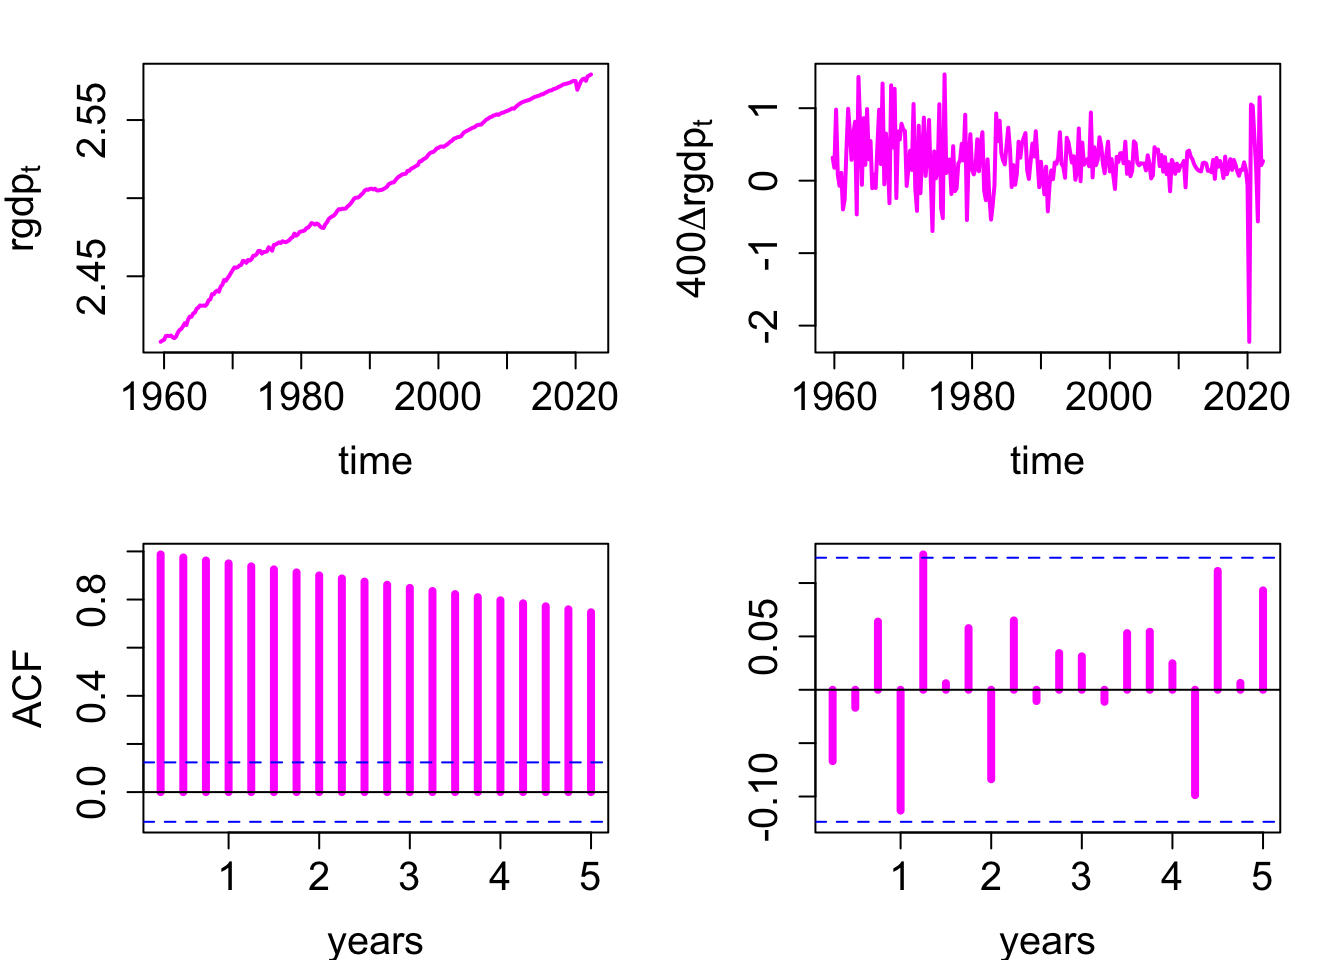
\includegraphics{./regression_exercises_files/figure-pdf/unnamed-chunk-3-1.pdf}

}

\end{figure}

Time series of annualized log-returns of the real GDP,
\(r_t = 400\Delta rgdp_t\), has very different properties. It is visible
in the data plot that the series oscillates around a positive constant
value. This fact, together with the evidence of hardly any serial
correlation from the autocorrelogram allows us to conclude that these
log returns are unit-root stationary series. Therefore, it seems that
the variable \(rgdp_t\) is intgrated of order 1. Finally, the time
series plot of the log-returns indicates higher volatility throughout
the half of the sample period than in the second one.

\hypertarget{exercise-4.2.-estimation-results}{%
\subsection*{Exercise 4.2. Estimation
results}\label{exercise-4.2.-estimation-results}}
\addcontentsline{toc}{subsection}{Exercise 4.2. Estimation results}

\begin{quote}
Set the parameters of the natural-conjugate prior distribution and
motivate the values that you choose. Use the computer codes you
developed in \textbf{Exercise 3.} to estimate the AR(1) model with a
constant term for each of the series. Use the obtained draws from the
posterior density to:

\begin{itemize}
\tightlist
\item
  Plot the Monte Carlo draws in trace plots. Comment on whether the
  algorithm converged to the stationary posterior distribution.
\item
  Plot the histograms of the marginal posterior distributions for all of
  the parameters of both the models that you estimated. Comment on the
  shapes of the histograms and the distribution of the probability mass.
\item
  Compute the sample means and sample standard deviations of the
  posterior draws for each of the estimated parameters. Interpret these
  values.
\end{itemize}
\end{quote}

\begin{Shaded}
\begin{Highlighting}[]
\NormalTok{priors.y }\OtherTok{=} \FunctionTok{list}\NormalTok{(}
  \AttributeTok{A    =} \FunctionTok{as.matrix}\NormalTok{(}\FunctionTok{c}\NormalTok{(}\DecValTok{0}\NormalTok{,}\DecValTok{1}\NormalTok{)),}
  \AttributeTok{V    =} \FunctionTok{diag}\NormalTok{(}\DecValTok{2}\NormalTok{),}
  \AttributeTok{s    =} \DecValTok{1}\NormalTok{,}
  \AttributeTok{nu   =} \DecValTok{3}
\NormalTok{)}
\NormalTok{priors.r }\OtherTok{=} \FunctionTok{list}\NormalTok{(}
  \AttributeTok{A    =} \FunctionTok{as.matrix}\NormalTok{(}\FunctionTok{c}\NormalTok{(}\DecValTok{0}\NormalTok{,}\DecValTok{0}\NormalTok{)),}
  \AttributeTok{V    =} \FunctionTok{diag}\NormalTok{(}\DecValTok{2}\NormalTok{),}
  \AttributeTok{s    =} \DecValTok{1}\NormalTok{,}
  \AttributeTok{nu   =} \DecValTok{3}
\NormalTok{)}

\NormalTok{posterior.y         }\OtherTok{=} \FunctionTok{ar1.posterior}\NormalTok{(y,priors.y)}
\NormalTok{posterior.draws.y   }\OtherTok{=} \FunctionTok{ar1.posterior.draws}\NormalTok{(}\AttributeTok{S=}\DecValTok{10000}\NormalTok{,posterior.y)}

\NormalTok{posterior.r         }\OtherTok{=} \FunctionTok{ar1.posterior}\NormalTok{(r,priors.r)}
\NormalTok{posterior.draws.r   }\OtherTok{=} \FunctionTok{ar1.posterior.draws}\NormalTok{(}\AttributeTok{S=}\DecValTok{10000}\NormalTok{,posterior.r)}
\end{Highlighting}
\end{Shaded}

The trace plots clearly indicate that the posterior draws for all of the
parameters of the models hover around constant values, that is, the
corresponding posterior means. No burn-in sample had to used for the
algorithm to obtain convergence. This is the expected outcome of direct
sampling from the posterior distributions in a known form.

\begin{Shaded}
\begin{Highlighting}[]
\FunctionTok{par}\NormalTok{(}\AttributeTok{mfrow=}\FunctionTok{c}\NormalTok{(}\DecValTok{3}\NormalTok{,}\DecValTok{2}\NormalTok{), }\AttributeTok{mar=}\FunctionTok{c}\NormalTok{(}\DecValTok{4}\NormalTok{,}\FloatTok{4.5}\NormalTok{,}\DecValTok{2}\NormalTok{,}\DecValTok{2}\NormalTok{),}\AttributeTok{cex.axis=}\FloatTok{1.5}\NormalTok{, }\AttributeTok{cex.lab=}\FloatTok{1.5}\NormalTok{)}
\FunctionTok{plot.ts}\NormalTok{(posterior.draws.y[,}\DecValTok{1}\NormalTok{], }\AttributeTok{main=}\FunctionTok{expression}\NormalTok{(rgdp[t]),}\AttributeTok{xlab=}\StringTok{""}\NormalTok{, }\AttributeTok{ylab=}\FunctionTok{expression}\NormalTok{(mu), }\AttributeTok{col=}\StringTok{"magenta"}\NormalTok{)}
\FunctionTok{plot.ts}\NormalTok{(posterior.draws.r[,}\DecValTok{1}\NormalTok{], }\AttributeTok{main=}\FunctionTok{expression}\NormalTok{(}\DecValTok{400}\SpecialCharTok{*}\NormalTok{Delta}\SpecialCharTok{*}\NormalTok{rgdp[t]),}\AttributeTok{xlab=}\StringTok{""}\NormalTok{, }\AttributeTok{ylab=}\StringTok{""}\NormalTok{, }\AttributeTok{col=}\StringTok{"magenta"}\NormalTok{)}
\FunctionTok{plot.ts}\NormalTok{(posterior.draws.y[,}\DecValTok{2}\NormalTok{], }\AttributeTok{main=}\StringTok{""}\NormalTok{,}\AttributeTok{xlab=}\StringTok{""}\NormalTok{, }\AttributeTok{ylab=}\FunctionTok{expression}\NormalTok{(alpha[}\DecValTok{1}\NormalTok{]), }\AttributeTok{col=}\StringTok{"magenta"}\NormalTok{)}
\FunctionTok{plot.ts}\NormalTok{(posterior.draws.r[,}\DecValTok{2}\NormalTok{], }\AttributeTok{main=}\StringTok{""}\NormalTok{,}\AttributeTok{xlab=}\StringTok{""}\NormalTok{, }\AttributeTok{ylab=}\StringTok{""}\NormalTok{, }\AttributeTok{col=}\StringTok{"magenta"}\NormalTok{)}
\FunctionTok{plot.ts}\NormalTok{(posterior.draws.y[,}\DecValTok{3}\NormalTok{], }\AttributeTok{main=}\StringTok{""}\NormalTok{,}\AttributeTok{xlab=}\StringTok{""}\NormalTok{, }\AttributeTok{ylab=}\FunctionTok{expression}\NormalTok{(sigma}\SpecialCharTok{\^{}}\DecValTok{2}\NormalTok{), }\AttributeTok{col=}\StringTok{"magenta"}\NormalTok{)}
\FunctionTok{plot.ts}\NormalTok{(posterior.draws.r[,}\DecValTok{3}\NormalTok{], }\AttributeTok{main=}\StringTok{""}\NormalTok{,}\AttributeTok{xlab=}\StringTok{""}\NormalTok{, }\AttributeTok{ylab=}\StringTok{""}\NormalTok{, }\AttributeTok{col=}\StringTok{"magenta"}\NormalTok{)}
\end{Highlighting}
\end{Shaded}

\begin{figure}[H]

{\centering 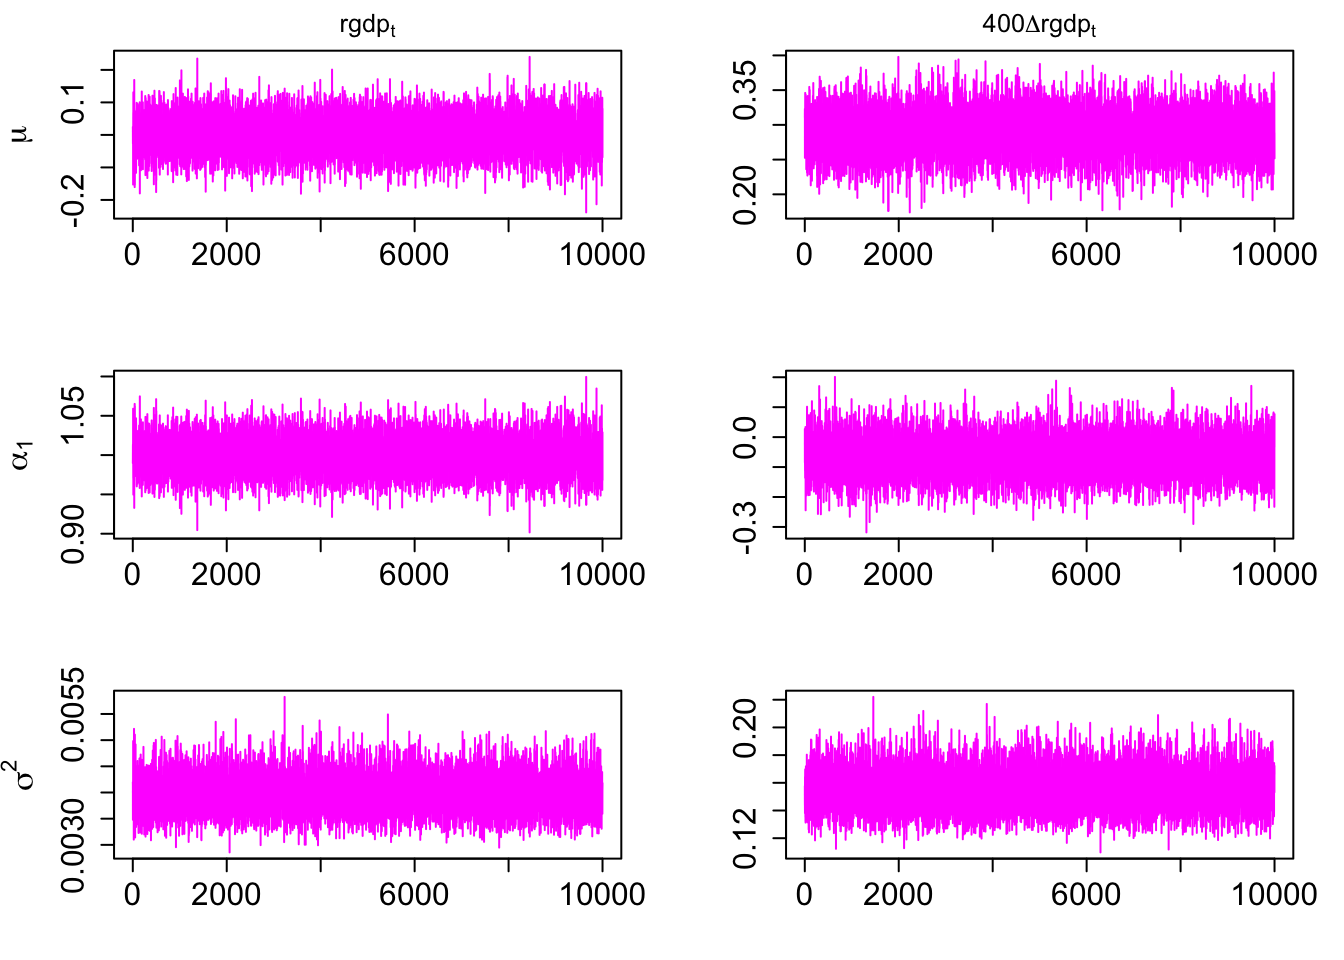
\includegraphics{./regression_exercises_files/figure-pdf/unnamed-chunk-5-1.pdf}

}

\end{figure}

The figure below presents histograms of the marginal posterior
distributions for the parameters of the models. The constant term and
the autoregressive parameters of both of the models have bell-shaped
distributions resembling the shape of t-distributed random variables,
while the error term variances' histograms are asymmetric to the right,
clearly reflecting the shape of the inverse gamma 2 distributions.

\begin{Shaded}
\begin{Highlighting}[]
\FunctionTok{par}\NormalTok{(}\AttributeTok{mfrow=}\FunctionTok{c}\NormalTok{(}\DecValTok{3}\NormalTok{,}\DecValTok{2}\NormalTok{), }\AttributeTok{mar=}\FunctionTok{c}\NormalTok{(}\DecValTok{4}\NormalTok{,}\FloatTok{4.5}\NormalTok{,}\DecValTok{2}\NormalTok{,}\DecValTok{2}\NormalTok{),}\AttributeTok{cex.axis=}\FloatTok{1.5}\NormalTok{, }\AttributeTok{cex.lab=}\FloatTok{1.5}\NormalTok{)}
\FunctionTok{hist}\NormalTok{(posterior.draws.y[,}\DecValTok{1}\NormalTok{], }\AttributeTok{main=}\FunctionTok{expression}\NormalTok{(rgdp[t]),}\AttributeTok{xlab=}\StringTok{""}\NormalTok{, }\AttributeTok{ylab=}\FunctionTok{expression}\NormalTok{(mu), }\AttributeTok{col=}\StringTok{"magenta"}\NormalTok{,}\AttributeTok{breaks=}\DecValTok{50}\NormalTok{)}
\FunctionTok{hist}\NormalTok{(posterior.draws.r[,}\DecValTok{1}\NormalTok{], }\AttributeTok{main=}\FunctionTok{expression}\NormalTok{(}\DecValTok{400}\SpecialCharTok{*}\NormalTok{Delta}\SpecialCharTok{*}\NormalTok{rgdp[t]),}\AttributeTok{xlab=}\StringTok{""}\NormalTok{, }\AttributeTok{ylab=}\StringTok{""}\NormalTok{, }\AttributeTok{col=}\StringTok{"magenta"}\NormalTok{,}\AttributeTok{breaks=}\DecValTok{50}\NormalTok{)}
\FunctionTok{hist}\NormalTok{(posterior.draws.y[,}\DecValTok{2}\NormalTok{], }\AttributeTok{main=}\StringTok{""}\NormalTok{,}\AttributeTok{xlab=}\StringTok{""}\NormalTok{, }\AttributeTok{ylab=}\FunctionTok{expression}\NormalTok{(alpha[}\DecValTok{1}\NormalTok{]), }\AttributeTok{col=}\StringTok{"magenta"}\NormalTok{,}\AttributeTok{breaks=}\DecValTok{50}\NormalTok{)}
\FunctionTok{hist}\NormalTok{(posterior.draws.r[,}\DecValTok{2}\NormalTok{], }\AttributeTok{main=}\StringTok{""}\NormalTok{,}\AttributeTok{xlab=}\StringTok{""}\NormalTok{, }\AttributeTok{ylab=}\StringTok{""}\NormalTok{, }\AttributeTok{col=}\StringTok{"magenta"}\NormalTok{,}\AttributeTok{breaks=}\DecValTok{50}\NormalTok{)}
\FunctionTok{hist}\NormalTok{(posterior.draws.y[,}\DecValTok{3}\NormalTok{], }\AttributeTok{main=}\StringTok{""}\NormalTok{,}\AttributeTok{xlab=}\StringTok{""}\NormalTok{, }\AttributeTok{ylab=}\FunctionTok{expression}\NormalTok{(sigma}\SpecialCharTok{\^{}}\DecValTok{2}\NormalTok{), }\AttributeTok{col=}\StringTok{"magenta"}\NormalTok{,}\AttributeTok{breaks=}\DecValTok{50}\NormalTok{)}
\FunctionTok{hist}\NormalTok{(posterior.draws.r[,}\DecValTok{3}\NormalTok{], }\AttributeTok{main=}\StringTok{""}\NormalTok{,}\AttributeTok{xlab=}\StringTok{""}\NormalTok{, }\AttributeTok{ylab=}\StringTok{""}\NormalTok{, }\AttributeTok{col=}\StringTok{"magenta"}\NormalTok{,}\AttributeTok{breaks=}\DecValTok{55}\NormalTok{)}
\end{Highlighting}
\end{Shaded}

\begin{figure}[H]

{\centering 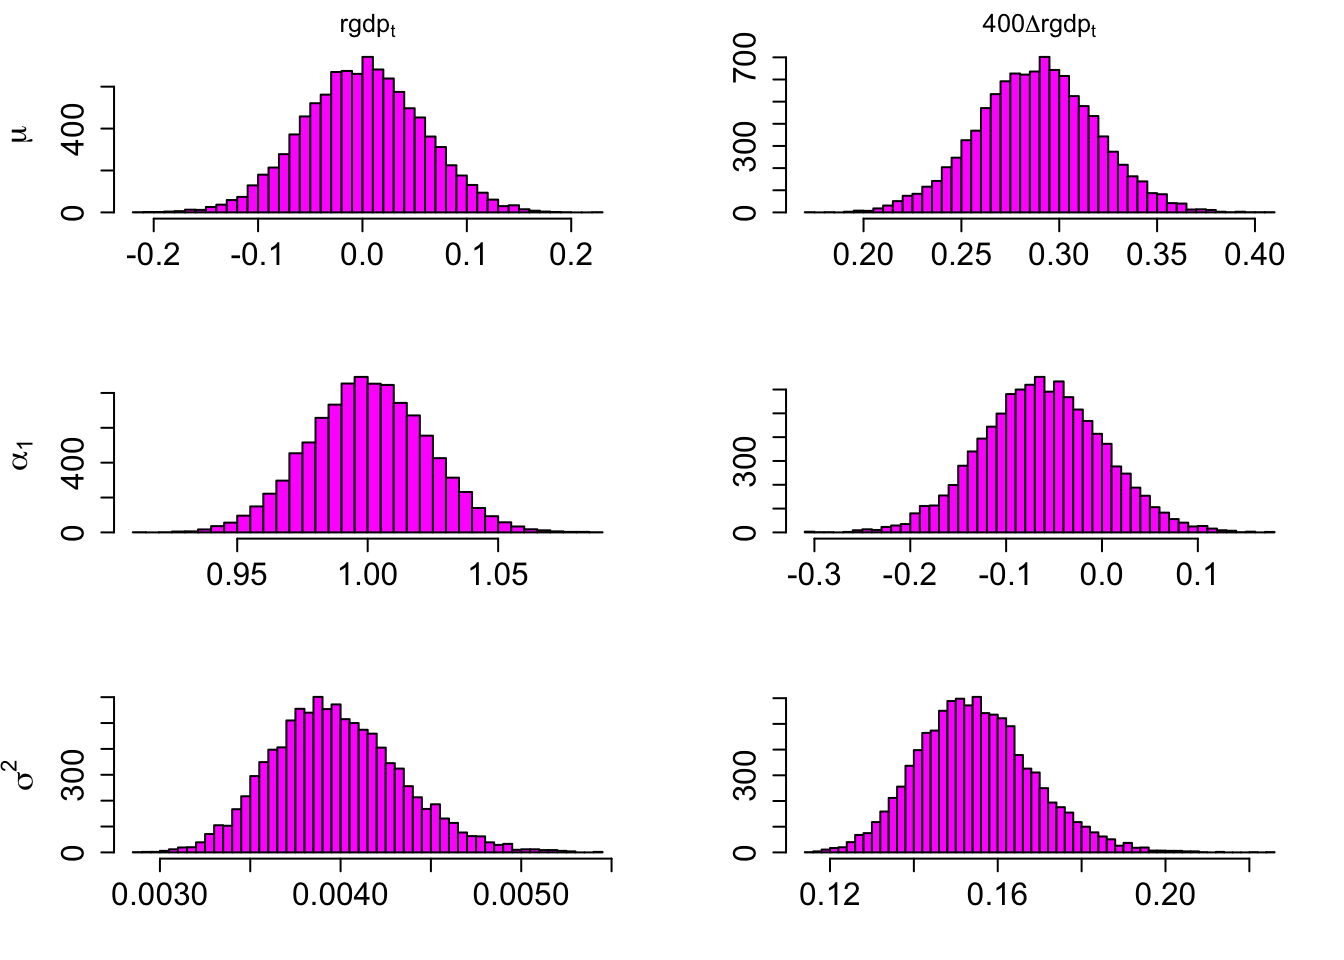
\includegraphics{./regression_exercises_files/figure-pdf/unnamed-chunk-6-1.pdf}

}

\end{figure}

The results below confirm the conclusions that could be formed about the
location of the probability mass of the parameters. The posterior mean
of the constant term of the model for variable \(rgdp_t\) is small and
point zero lays in a region of high concentration of the probability
mass. For the same model, the autoregressive slope has the value of
nearly one and the shape of the posterior distribution is typical for a
unit-root non-stationary random variable. The non-stationarity is well
documented by the results above, however, a hypothesis of non-zero drift
does not find empirical support.

\begin{Shaded}
\begin{Highlighting}[]
\FunctionTok{round}\NormalTok{(}\FunctionTok{rbind}\NormalTok{(}
  \FunctionTok{apply}\NormalTok{(posterior.draws.y,}\DecValTok{2}\NormalTok{,mean),}
  \FunctionTok{apply}\NormalTok{(posterior.draws.y,}\DecValTok{2}\NormalTok{,sd)}
\NormalTok{),}\DecValTok{4}\NormalTok{)}
\end{Highlighting}
\end{Shaded}

\begin{verbatim}
       [,1]   [,2]  [,3]
[1,] 0.0002 1.0002 4e-03
[2,] 0.0562 0.0225 4e-04
\end{verbatim}

\begin{Shaded}
\begin{Highlighting}[]
\FunctionTok{round}\NormalTok{(}\FunctionTok{rbind}\NormalTok{(}
  \FunctionTok{apply}\NormalTok{(posterior.draws.r,}\DecValTok{2}\NormalTok{,mean),}
  \FunctionTok{apply}\NormalTok{(posterior.draws.r,}\DecValTok{2}\NormalTok{,sd)}
\NormalTok{),}\DecValTok{4}\NormalTok{)}
\end{Highlighting}
\end{Shaded}

\begin{verbatim}
       [,1]    [,2]   [,3]
[1,] 0.2878 -0.0620 0.1548
[2,] 0.0299  0.0632 0.0139
\end{verbatim}

The autoregressive slope parameter for the model for the quarterly
annualized log-returns has the posterior distribution concentrated near
value zero with the posterior mean equal to -0.063 and the posterior
standard deviation equal to 0.07. Therefore, this variable is clearly
stationary, mean-reverting, and the average quarterly annualized
log-return has value around 3.6 pp.

\hypertarget{exercise-4.3.-unit-root-testing}{%
\subsection*{Exercise 4.3. Unit root
testing}\label{exercise-4.3.-unit-root-testing}}
\addcontentsline{toc}{subsection}{Exercise 4.3. Unit root testing}

\begin{quote}
Compute the fraction of the posterior draws of parameter \(\alpha_1\)
that are greater than 1 for both of the models. Confront these results
with the histograms, posterior means and standard deviations of
\(\alpha_1\) for both of the models, and interpret these results.
Comment on the Bayesian evidence in favour of the unit root hypothesis
for each of the time series. Comment on the interpretations of the
values of the constant term in both of the models in the context of your
statements on unit-root stationarity of the considered time series.
\end{quote}

The table below reports also the posterior probabilities that parameter
\(\alpha_1\) has value greater than 1 for both of the models. These
probabilities take values of 0.47 and 0 respectively and clearly confirm
the statements regarding the unit-root non-stationarity of both of the
variables. The former values indicates that no statistical test based on
the estimates above would reject the hypothesis of unit-root in
\(rgdp_t\) while such a hypothesis would clearly be rejected for the
log-returns.

\begin{Shaded}
\begin{Highlighting}[]
\FunctionTok{sum}\NormalTok{(posterior.draws.y[,}\DecValTok{2}\NormalTok{]}\SpecialCharTok{\textgreater{}}\DecValTok{1}\NormalTok{)}\SpecialCharTok{/}\DecValTok{10000}
\end{Highlighting}
\end{Shaded}

\begin{verbatim}
[1] 0.5007
\end{verbatim}

\begin{Shaded}
\begin{Highlighting}[]
\FunctionTok{sum}\NormalTok{(posterior.draws.r[,}\DecValTok{2}\NormalTok{]}\SpecialCharTok{\textgreater{}}\DecValTok{1}\NormalTok{)}\SpecialCharTok{/}\DecValTok{10000}
\end{Highlighting}
\end{Shaded}

\begin{verbatim}
[1] 0
\end{verbatim}



\end{document}
